% ==============================================================================
\chapter{Active edge sensors}
\label{ch:ActiveEdgeSensors}
% ==============================================================================    

Active-edge technology allows for seamless tiling of pixel sensors by
depleting the sensors up to their physical edges. This allows for high
coverage without creating overlaps between the pixel sensors and
therefore reduces the material budget in the detector. The process
consists of extending the backside implantation to the edge.

This technology is particularly interesting for the CLIC vertex
detector where the material budget is constrained to be only
$0.2\%$~X\textsubscript{0}. The ladders of pixel detectors can be made
without overlaps and with a high coverage.

In this chapter, the fabrication process for active edge sensors is
described. Planar sensors produced by Advacam~\cite{AdvacamRef} and
bump bonded to Timepix3 ASICs are tested in test beams. The signal
collection and the efficiency on the edge is presented. The test beam
results are compared to TCAD simulations.

%% --------------------------------------------- %%
\section{The active-edge technology processing}

Thin $50-150\,\micron$ thick n-in-p planar sensors with active edges
have been produced by Advacam~\cite{AdvacamRef} using a Deep Reactive
Ion Etching (DRIE) process. The DRIE process is used to make trenches
around the sensors and allows for extending the back-side
implantation, and thereby the bias voltage, to the edge of the sensor
by doping the sensor sides. The gradient of potential between the edge
and the last pixel can be very high and could lead to a breakdown of
the sensor. A guard ring (GR) consists of an n-implant with a metallic
contact on top of it surrounding the pixel matrix close to the edge
and thereby smoothening the potential transition between the edge and
the neighbouring pixels. The guard ring can be kept floating or
grounded by connecting it to the ground of the readout ASIC.

The active-edge sensors are bump bonded to Timepix3 readout chips
($55\,\micron$ pixel pitch) and studied in test beams and
simulations. Timepix3 ASICs provide an extra row of bumped pixels
allowing to connect the guard ring to ground
potential. Figure~\ref{fig:activeedge} shows a cross section of an
active-edge sensor with and without guard ring.


\begin{figure}[htbp]
  \centering
  \begin{subfigure}[b]{0.45\textwidth}
    \begin{tikzpicture}
      \node[anchor=south west,inner sep=0] (image) at
      (0,0){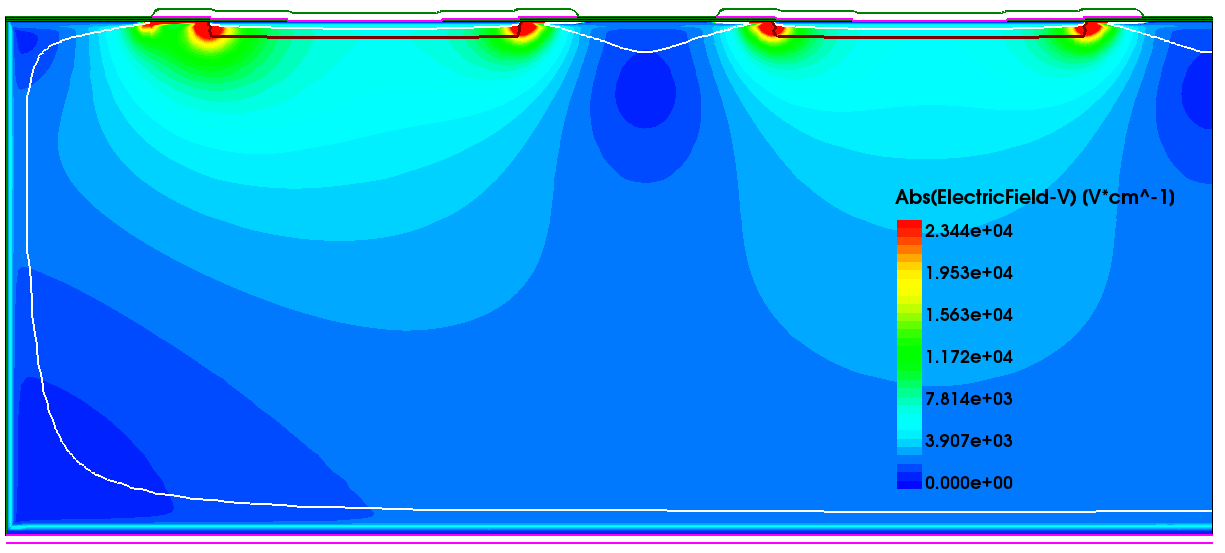
\includegraphics[width=\textwidth]{figures/ActiveEdge/Efield_20_NGR.png}};
      \begin{scope}[x={(image.south east)},y={(image.north west)}]
        \draw[-, dashed, line width=.7pt, color=white](0.1, 0.05) -- (0.1, 0.92);
        \draw[-, dashed, line width=.7pt, color=white](0.54, 0.05) -- (0.54, 0.92);
        
        \draw[<->, line width=.7pt, color=black](0.01, 1) -- (0.16, 1); % edge width
        \node[above, color=black] at (0.05, 1) {edge};
        
        \draw[<->, thick, color=black](0.17, 1) -- (0.43, 1); % n-implant
        \node[above, color=black] at (0.33, 1) {n-implant};

        \node[above, color=white] at (0.3, 0.5) {\textbf{p-substrate}};
        \draw[<->, thick, color=black](0.54, 0.0) -- (0.98, 0.0); % pixel width
        \node[below, color=black] at (0.75, 0.0) {pixel (55 \micron)};
        
        \draw[-, line width=3pt, color=violet](0.0, 0.05) -- (0.98, 0.05); % p+ backside contact
        \node[below, color=violet] at (0.15, 0.0) {p+ backside contact};
        \draw[-, line width=3pt, color=violet](0.0, 0.045) -- (0.0, 0.93); % p+ active-edge contact
        \node[left, color=violet, rotate=90] at (-0.05, 0.7) {p+ active edge};
        % \node[left, color=white, rotate=90] at (0.08, 0.9) {\textbf{final pixel edge}};

        % \draw[help lines,xstep=.1,ystep=.1] (0, 0) grid (1,1);
        % \foreach \x in {0,1,...,9} { \node [anchor=north] at (\x/10,0) {0.\x}; }
        % \foreach \y in {0,1,...,9} { \node [anchor=east] at (0,\y/10) {0.\y}; }

      \end{scope}
    \end{tikzpicture}
    \caption{No guard ring}
  \end{subfigure}\hfill
  \begin{subfigure}[b]{0.45\textwidth}
    \begin{tikzpicture}
      \node[anchor=south west,inner sep=0] (image) at
      (0,0){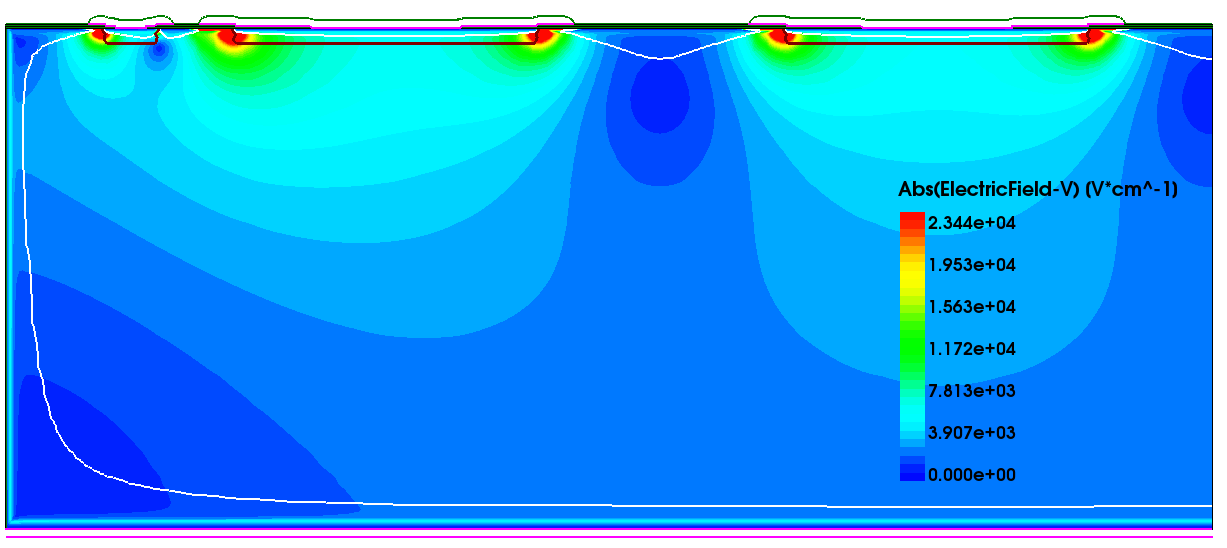
\includegraphics[width=\textwidth]{figures/ActiveEdge/Efield_23_FGR.png}};
      \begin{scope}[x={(image.south east)},y={(image.north west)}]
        \draw[-, dashed, line width=.7pt, color=white](0.14, 0.05) -- (0.14, 0.92);
        \draw[-, dashed, line width=.7pt, color=white](0.54, 0.05) -- (0.54, 0.92);
        \draw[<->, line width=.7pt, color=black](0.01, 1) -- (0.16, 1); % edge width
        
        \node[above, color=black] at (0.1, 1) {edge};
        \node[above, color=white] at (0.1, 0.75) {\textbf{GR}};
        \node[above, color=white] at (0.3, 0.5) {\textbf{p-substrate}};
        \draw[<->, line width=.4pt, color=black](0.54, 0.0) -- (0.98, 0.0); % pixel width
        \node[below, color=black] at (0.75, 0.0) {\small{pixel (55
            \micron)}};

        \draw[<->, thick, color=black](0.19, 1) -- (0.44, 1); % n-implant
        \node[above, color=black] at (0.33, 1) {n-implant};
        
        \draw[-, line width=3pt, color=violet](0.01, 0.05) -- (0.99, 0.05); % p+ backside contact
        \draw[-, line width=3pt, color=violet](0.01, 0.045) -- (0.01, 0.95); % p+ active-edge contact
        % \draw[help lines,xstep=.1,ystep=.1] (0, 0) grid (1,1);
        % \foreach \x in {0,1,...,9} { \node [anchor=north] at (\x/10,0) {0.\x}; }
        % \foreach \y in {0,1,...,9} { \node [anchor=east] at (0,\y/10) {0.\y}; }
      \end{scope}
    \end{tikzpicture}
    \caption{With guard ring}
  \end{subfigure}
  \caption{Schematic showing the cross section of a $50\,\micron$
    thick sensor with active-edge technology. The pixel grid
    considered in the analysis is indicated with dashed lines. The
    electric field distribution obtained from a TCAD simulation with a
    bias voltage of 15~V is also illustrated. (a) does not contain any
    guard ring (GR) and (b) contains a guard ring in the edge which
    consists of an n-implant with a metallic contact on top of it.}
  \label{fig:activeedge}
\end{figure}

%% --------------------------------------------- %%
\newpage
\subsection{Process flow for sensor production by Advacam}
\label{sec:AdvacamProcessFlow}

The process flow used by Advacam to produce active-edge sensors is
schematically illustrated in \cref{fig:AdvacamProcessFlow} and
described as follows~\cite{AdvacamProcessFlow}.

\begin{enumerate}
\item First, the backside implantation is done by doping the detector
  wafer with phosphorus.
\item The wafer is then bonded to a support wafer to perform the next
  steps.
\item By grinding and CMP (Chemical-mechanical planarisation)
  polishing the final detector thickness is obtained.
\item The doping for the pixels and also the guard rings are
  implanted.
\item The DRIE etching is performed to uncover the edges of the
  detector.
\item Ions are implanted to the sidewalls of the sensor to activate
  the edges.
\item Annealing of the sensor in order to activate the dopants and
  oxidation of the edges.
\item The opening of the contacts for the Aluminum patterning and the
  deposition of the UBM layer for the pixels and guard rings.
\item The support wafer is finally removed and the backside metal is
  deposited. The sensor is ready to be bump bonded to the readout
  chip.
\end{enumerate}


\begin{figure}[htbp]
  \centering
  \begin{subfigure}[b]{0.3\textwidth}
    \centering
    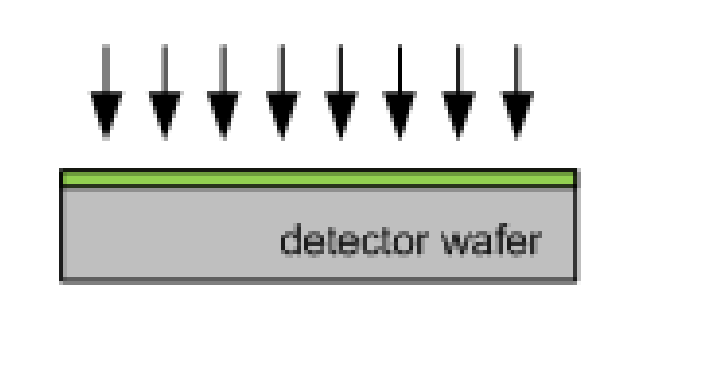
\includegraphics[width=\textwidth]{figures/ActiveEdge/advacamProcess/wafer_1}
    \caption{}
  \end{subfigure}\hfill
  \begin{subfigure}[b]{0.3\textwidth}
    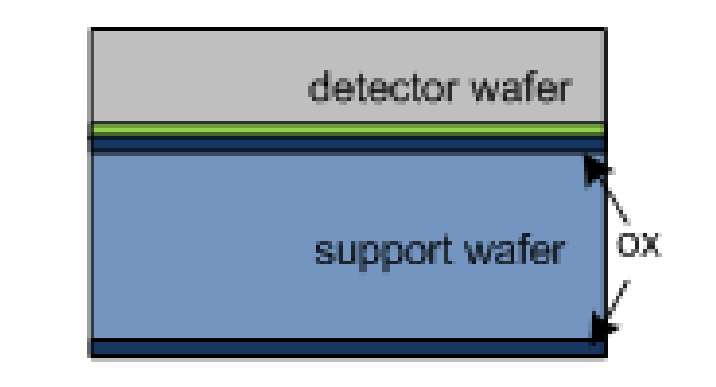
\includegraphics[width=\textwidth]{figures/ActiveEdge/advacamProcess/wafer_2}
    \caption{}
  \end{subfigure}\hfill
  \begin{subfigure}[b]{0.3\textwidth}
    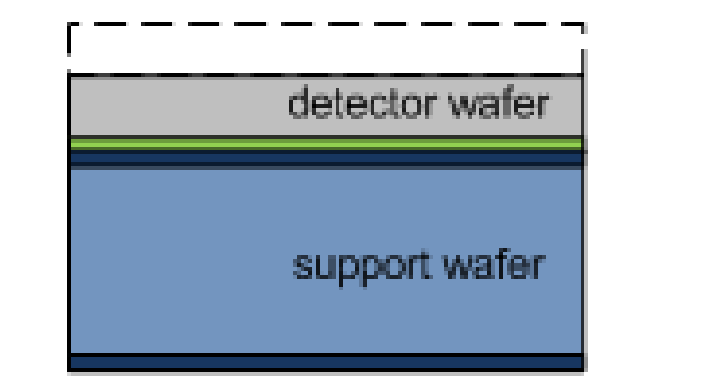
\includegraphics[width=\textwidth]{figures/ActiveEdge/advacamProcess/wafer_3}
    \caption{}
  \end{subfigure}\\

  \begin{subfigure}[b]{0.3\textwidth}
    \centering
    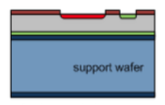
\includegraphics[width=\textwidth]{figures/ActiveEdge/advacamProcess/wafer_4}
    \caption{}
  \end{subfigure}\hfill
  \begin{subfigure}[b]{0.3\textwidth}
    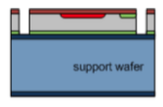
\includegraphics[width=\textwidth]{figures/ActiveEdge/advacamProcess/wafer_5}
    \caption{}
  \end{subfigure}\hfill
  \begin{subfigure}[b]{0.3\textwidth}
    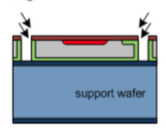
\includegraphics[width=\textwidth]{figures/ActiveEdge/advacamProcess/wafer_6}
    \caption{}
  \end{subfigure} \\

  \begin{subfigure}[b]{0.3\textwidth}
    \centering
    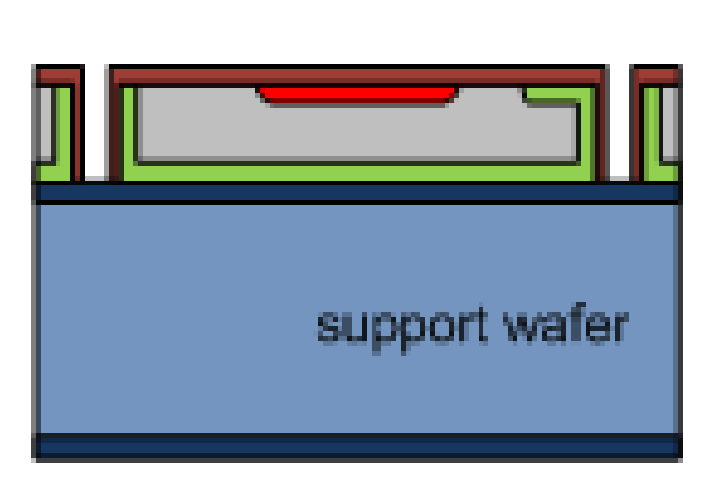
\includegraphics[width=\textwidth]{figures/ActiveEdge/advacamProcess/wafer_7}
    \caption{}
  \end{subfigure}\hfill
  \begin{subfigure}[b]{0.3\textwidth}
    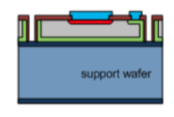
\includegraphics[width=\textwidth]{figures/ActiveEdge/advacamProcess/wafer_8}
    \caption{}
  \end{subfigure}\hfill
  \begin{subfigure}[b]{0.3\textwidth}
    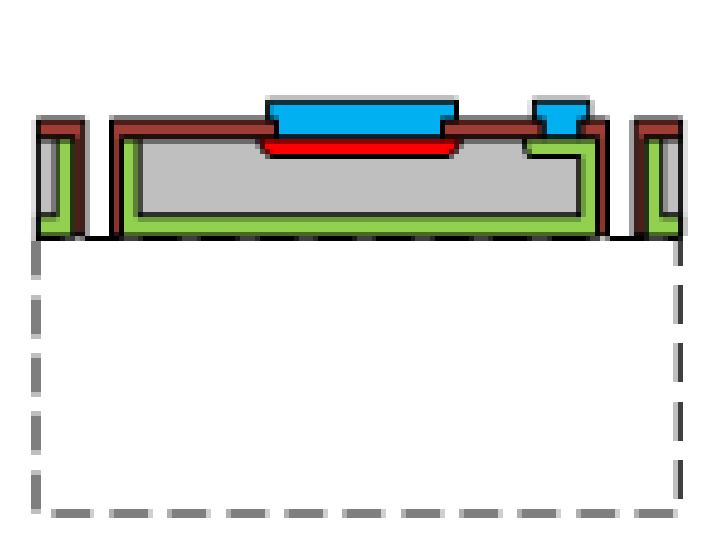
\includegraphics[width=\textwidth]{figures/ActiveEdge/advacamProcess/wafer_9}
    \caption{}
  \end{subfigure}

  \caption{Schematic illustration of the process flow for the
    fabrication of active edge sensors by
    Advacam~\cite{AdvacamProcessFlow}.}
  \label{fig:AdvacamProcessFlow}
\end{figure}


%% --------------------------------------------- %%
\newpage
\subsection{Layout parameters of produced assemblies}
\label{sec:AEgeometry}

The produced assemblies by Advacam and tested in test beams are listed
in \cref{tab:Timepix3Assemblies}. The edge distance is defined by the
distance between the last pixel implant and the physical sensor
edge. The layouts of the assemblies are shown in
\cref{fig:Layout_guard_ring} and the colors defining the different
sensor layers are described in
\cref{fig:PixelLayout,tab:PixelStackDimensions}. The same convention
is also used for describing the layers for the guard
ring. \cref{tab:DimensionsForAssemblies} summarises the dimensions of
the implants for the sensors. These dimensions are used for the
implementation of the sensors in TCAD simulations.


\begin{figure}[htbp]
  \begin{subfigure}[t]{0.5\textwidth}
    \centering
    \begin{tikzpicture}
      \node[anchor=south west,inner sep=0] at
      (0,0){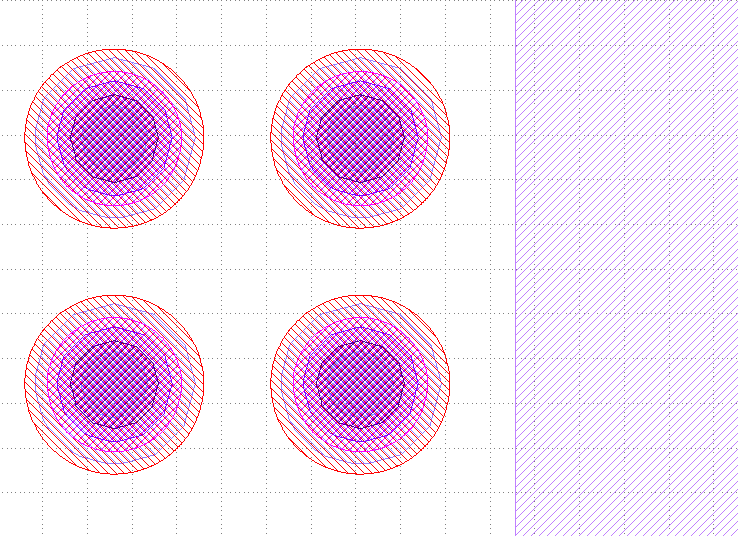
\includegraphics[width=0.8\textwidth]{figures/ActiveEdge/geometry_20NGR.png}};

      \begin{scope}[x={(image.south east)},y={(image.north west)}]

        \draw[blue, thick](0.62, 0.1)--(0. 62, 0.7);
        \draw[blue, thick, dashed](0.58, 0.1)--(0.58, 0.7);
        \draw[blue, thick, dashed](0.3, 0.1)--(0.3, 0.7);

        \draw[blue, thick, dashed](0.3, 0.1)--(0.62, 0.1);
        \draw[blue, thick, dashed](0.3, 0.7)--(0.62, 0.7);

        \node[below, color=blue] at (0.3, 0.1) {-0.055 mm};
        \node[below, color=blue] at (0.58, 0.1) {0 mm};

        \draw[<->, blue, thick](0.51, 0.4)--(0.62, 0.4);
        \node[right, color=blue] at (0.62, 0.4) {Edge distance};

      \end{scope}
    \end{tikzpicture}
    \caption{20-NGR}
    \label{fig:Layout20_NGR}
  \end{subfigure}~
  \begin{subfigure}[t]{0.5\textwidth}
    \centering
    \begin{tikzpicture}
      \node[anchor=south west,inner sep=0] at
      (0,0){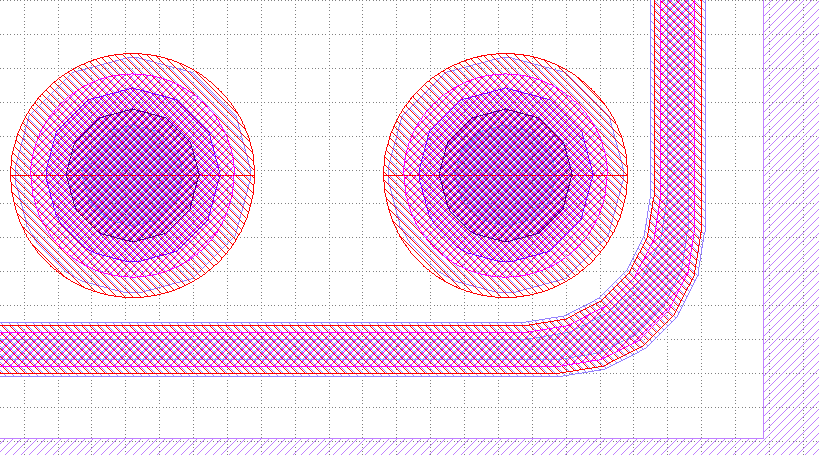
\includegraphics[width=0.8\textwidth]{figures/ActiveEdge/geometry_23FGR.png}};
    \end{tikzpicture}
    \caption{23-FGR}
    \label{fig:Layout20_FGR}
  \end{subfigure}
  \begin{subfigure}[t]{0.5\textwidth}
    \centering
    \begin{tikzpicture}
      \node[anchor=south west,inner sep=0] at
      (0,0){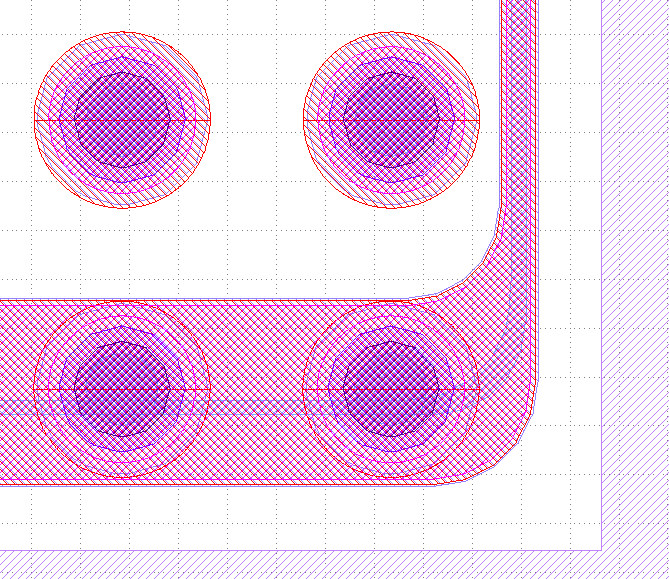
\includegraphics[width=0.55\textwidth]{figures/ActiveEdge/geometry_28GNDGR.png}};
    \end{tikzpicture}
    \caption{28-GNDGR}
    \label{fig:Layout20_GNDGR}
  \end{subfigure}~
  \begin{subfigure}[t]{0.5\textwidth}
    \centering
    \begin{tikzpicture}
      \node[anchor=south west,inner sep=0] at
      (0,0){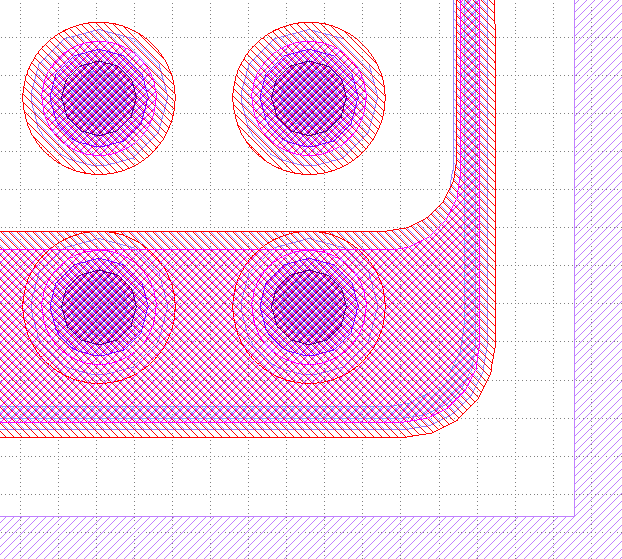
\includegraphics[width=0.55\textwidth]{{figures/ActiveEdge/geometry_55GNDGR.png}}};
    \end{tikzpicture}
    \caption{55-GNDGR, 55-GNDGR-100, 55-GNDGR-150}
    \label{fig:Layout50_GNDGR}
  \end{subfigure}~
  \caption{Sensor layouts for different guard-ring solutions for the
    assemblies described in \cref{tab:Timepix3Assemblies}. (a) shows
    the convention used in
    \cref{fig:20-NGR_eff_TOT,fig:23-FGR_eff_TOT,fig:28-GNDGR_eff_TOT,fig:55-GNDGR_eff_TOT,fig:55-GNDGR-100_eff_TOT,fig:55-GNDGR-150_eff_TOT}
    to express the efficiency and the charge distribution at the edge
    as a function of the track position. The border of the last pixel
    before the edge is indicated by a dashed line (at position 0 mm)
    and the physical sensor edge with a continuous line.}
  \label{fig:Layout_guard_ring}
\end{figure}


\begin{figure}[htbp]
  \centering
  \begin{minipage}[t]{.4\textwidth}
    \centering
    \vspace{0pt}
    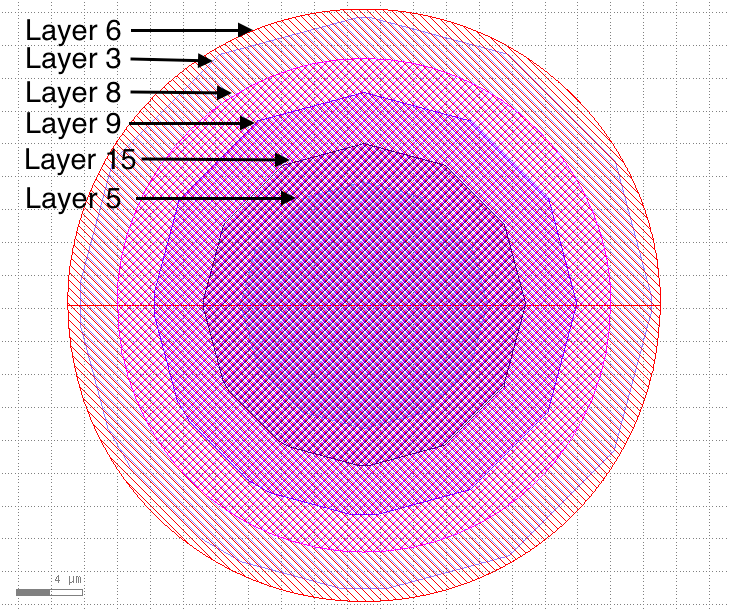
\includegraphics[width=0.95\textwidth]{figures/ActiveEdge/pixelLayout_withLayers.png}
    \caption{The different layers in the geometry description used for
      the sensor production.}
    \label{fig:PixelLayout}
  \end{minipage}
  \hfill
  \begin{minipage}[t]{.56\textwidth}
    \centering
    \vspace{0pt}
    \captionof{table}{Layers in the geometry description used for the
      sensor production (Picture from 23-FGR).}
    \label{tab:PixelStackDimensions}
    \begin{tabular}{l c c}
      \toprule
      Layer number & Layer \\
      \midrule
      6 & metal\\
      3 & implant \\
      8 & implant \\
      9 & UBM \\
      15 & passivation \\
      5 & contact to connect Al to Si \\
      \bottomrule
    \end{tabular}
  \end{minipage}
\end{figure}

\begin{table}
  \centering
  \captionof{table}{The dimensions of the different implants in for
    the sensors listed in \cref{tab:Timepix3Assemblies}. The
    edge distance is the distance between the last pixel implant to the physical edge of the sensor. The metal width
    is the diameter of the metal layer for the pixels. The doping width is the
    diameter of the pixel implant. The contact width is the diameter of
    the contact between silicon and the metal (where the oxide is
    etched). The GR offset is the distance between the physical edge of
    the sensor and the implant of the guard ring.}
  \label{tab:DimensionsForAssemblies}
  \begin{tabular}{l c c c c}
    \toprule
    & 20-NGR-50 & 23-FGR-50 & 28-GNDGR-50 & 55-GNDGR-50, 100, 150 \\
    \midrule
    Edge width [\micron] & 20 & 23 & 28 & 55 \\
    Metal width [\micron] & 40 & 36 & 36 & 40 \\
    Doping width [\micron] & 30 & 30 & 30 & 30 \\
    Contact width [\micron] & 15 & 15 & 15 & 15 \\
    GR offset [\micron] & - & 10 & 14.5 & 25 \\
    GR doping width [\micron] & - & 5 & 5 & 5 \\
    GR contact width [\micron] & - & 3 & 3 & 3 \\
    GR metal width [\micron] & - & 7 & 7 & 10 \\
    \bottomrule
  \end{tabular}
\end{table}

%% --------------------------------------------- %%
\newpage
\subsection{Process flow for the simulation of the active-edge designs}
\label{sec:processFlowTCAD}

TCAD simulations (c.f. \cref{sec:TCAD}) are used to simulate the
fabrication process and the device operation of active edge
sensors. The electric field and the electrostatic potential
distributions within the sensor are calculated. For realistic
simulations, the real dimensions of the assemblies as listed in
\cref{tab:DimensionsForAssemblies} are used. Due to the computational
power required for such simulations, the simulation is restricted to
two pixels in a 2D configuration.

The fabrication process of the sensors is simulated as follows:
\begin{enumerate}
\item The dimensions of the pixels, implants, contacts and metal
  layers are defined.
\item The meshing is refined at the borders of the sensor and around the
  implants based on the concentration of the dopants using an adaptive
  meshing with the command \texttt{refinebox}.
\item The silicon region is then defined for two pixels, the edge
  region and an extra silicon edge which will be etched later (to make
  the process more realistic). 
  %The silicon is doped with borons (p-type material) with the initial resistivity of $\rho=10~\text{k}\Omega\text{cm}$ ($4.41\times 10^{11}\,\inversecmcubic$).
\item First a layer of $0.2\,\micron$ thick oxide and then a layer of
  $0.2\,\micron$ thick nitride are deposited on the top of the sensor.
\item From the bias scan, the depletion voltage is measured for the
  assemblies (c.f. \cref{sec:ThinSensors_depletionVoltage}). Thus the
  silicon is doped with borons at a concentration of
  $1\times10^{12}\,\inversecmcubic$. The implantation is done with an
  energy of $180\,\kev$.
\item The nitride is then etched at the positions of the implants for
  the pixels and the guard ring if the assembly contains one. First a
  mask is put on the positions where the nitride is going to
  stay. Then the etching is done at the implantation
  positions. Phosphorus (n-type material) is implanted with a
  concentration of $1\times10^{15}\,\inversecmcubic$ with an energy of
  $120\,\kev$. Masks limit the etching and the deposition to a certain
  window and provide the possibility to imitate the lithographic
  patterning.
\item The extra edge (as explained in point 3) is etched to achieve
  the edge distance of the assembly. In this process, first the
  nitride layer, then the oxide and finally the silicon layers are
  etched.
\item The sensor is then flipped and a layer of oxide is deposited on
  the backside with a thickness of $0.04\,\micron$. Borons with a
  concentration of $1\times10^{15}\,\inversecmcubic$ and an energy of
  $60\,\kev$ are implanted. Then the oxide is etched from the backside
  and the sensor is flipped again to the initial position.
\item The oxide is then etched at the contact positions.
\item The meshing of the edge is then refined adaptively depending
  on the concentration of the ions and for a thickness of $1\,\micron$.
\item A photoresist is deposited on the top of the sensor with a
  thickness of $2\,\micron$.
\item Borons are implanted to the edge with a concentration of
  $1\times10^{15}\,\inversecmcubic$, an energy of $60\,\kev$ and a
  tilt of $15\degrees$.
\item The photoresist is then removed.
\item To activate the dopants, the sensor is annealed at a constant
  temperature of $940\degrees$C during 240 minutes.
\item The pixels and guard ring metal layer is deposited using an
  aluminium layer with a thickness of $0.8\,\micron$.
\item A layer of aluminium with a thickness of $0.8\,\micron$ is
  deposited for the contact of the high-voltage on the back-side of
  the sensor.
\end{enumerate}
 

The resulting doping concentration for the different layouts is shown
in Figure~\ref{fig:TCAD_dopingConcentration}.

%% --------------------------------------------- %%
\newpage
\section{Electrical measurements in laboratory and simulations}

\cref{fig:IVmeasurements} shows the measured leakage current in the
different assemblies as a function of the bias voltage at the room
temperature of $22^{\circ}$~C. The breakdown occurs earlier for the
assembly without guard ring (20-NGR-50) compared to the other
assemblies. For the nominal operation (at -15~V for $50\,\micron$,
-20~V for $100\,\micron$ and -30~V for $150\,\micron$ thick sensors),
none of the assemblies are operated beyond the breakdown voltage.

\cref{fig:IVmeasurements_TCAD} shows the leakage current obtained from
the TCAD simulations. The current calculated from the 2D simulation is
scaled to obtain the current in the total matrix. In TCAD simulations,
the sensor is simulated and the effect of the readout chip is not
included on the leakage current.

\begin{figure}[htbp]
  \centering
  \begin{subfigure}[b]{0.45\textwidth}
    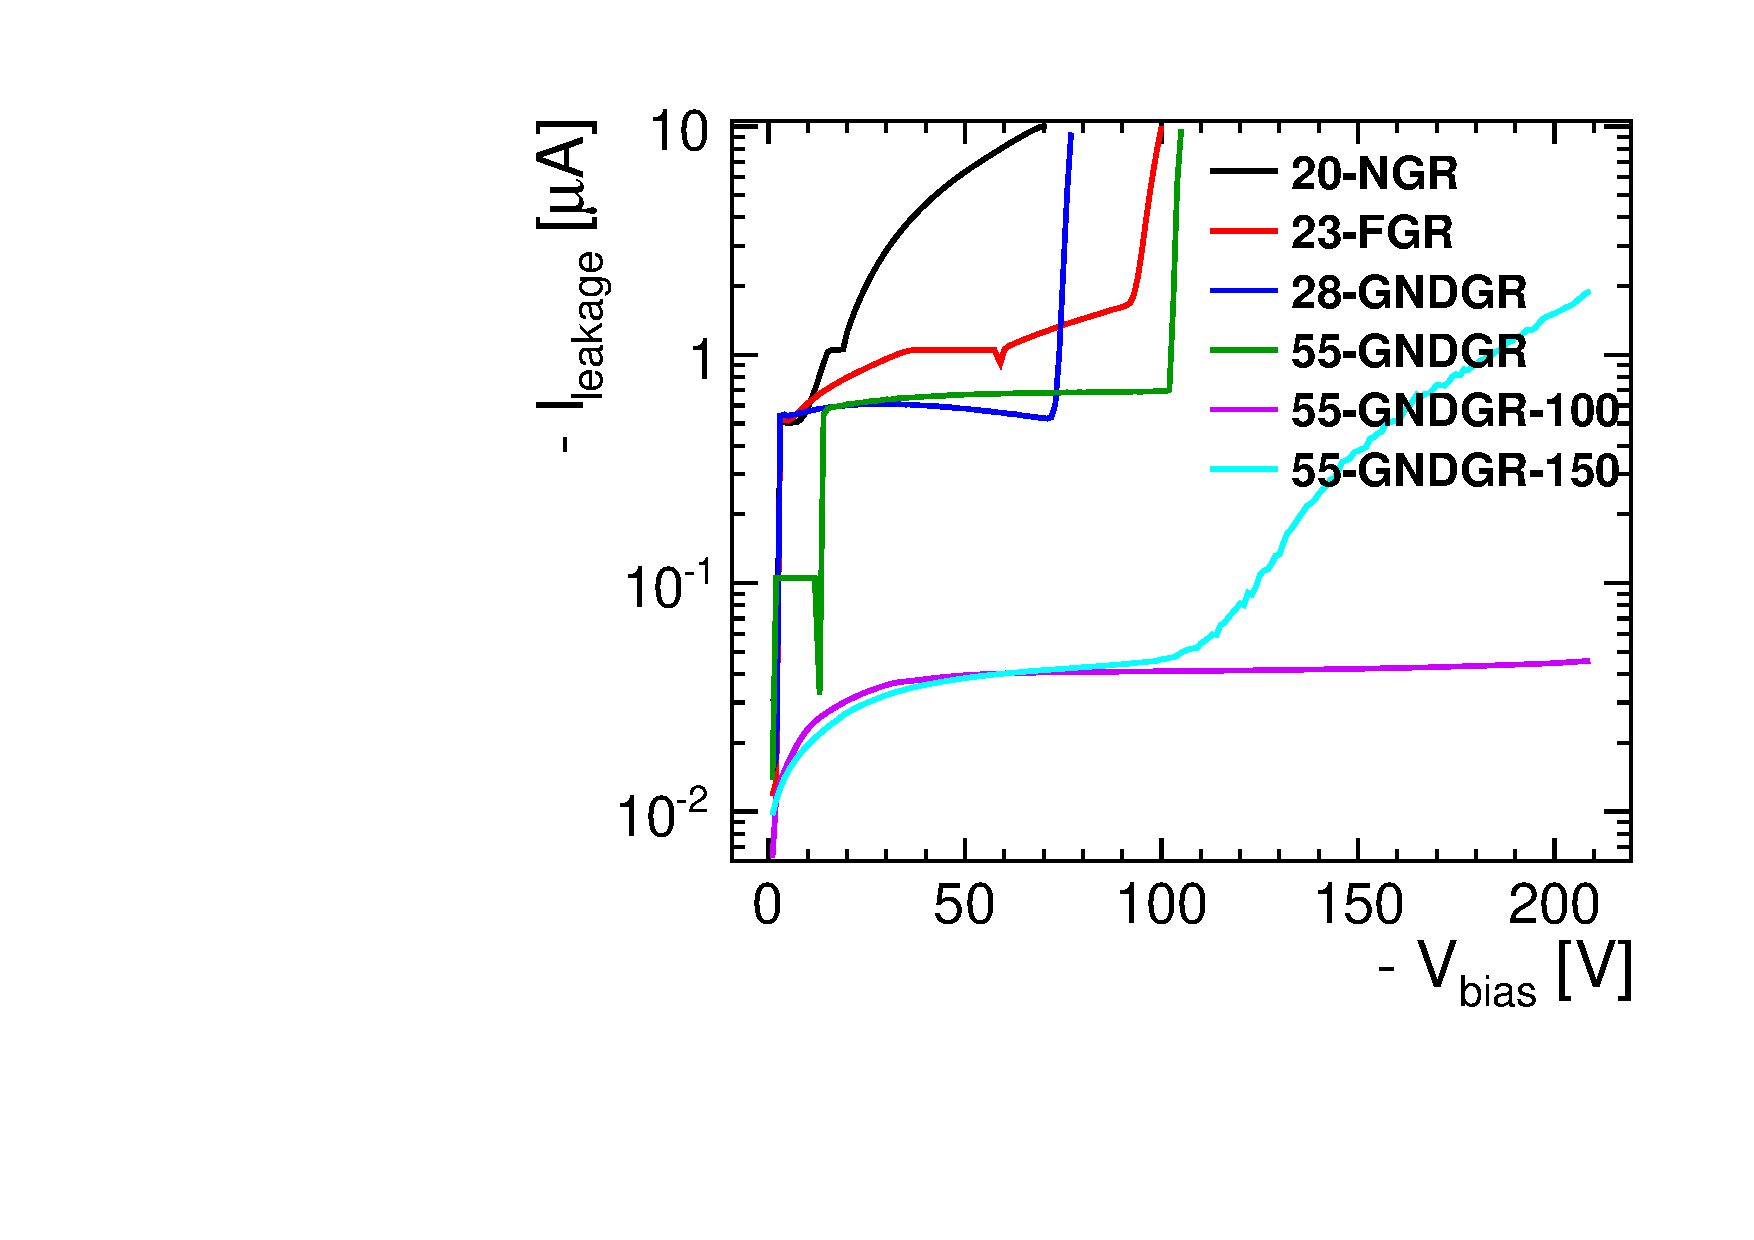
\includegraphics[width=\textwidth]{figures/ActiveEdge/IVCurve.pdf}
    \caption{}
    \label{fig:IVmeasurements}
  \end{subfigure}\hfill
  \begin{subfigure}[b]{0.45\textwidth}
    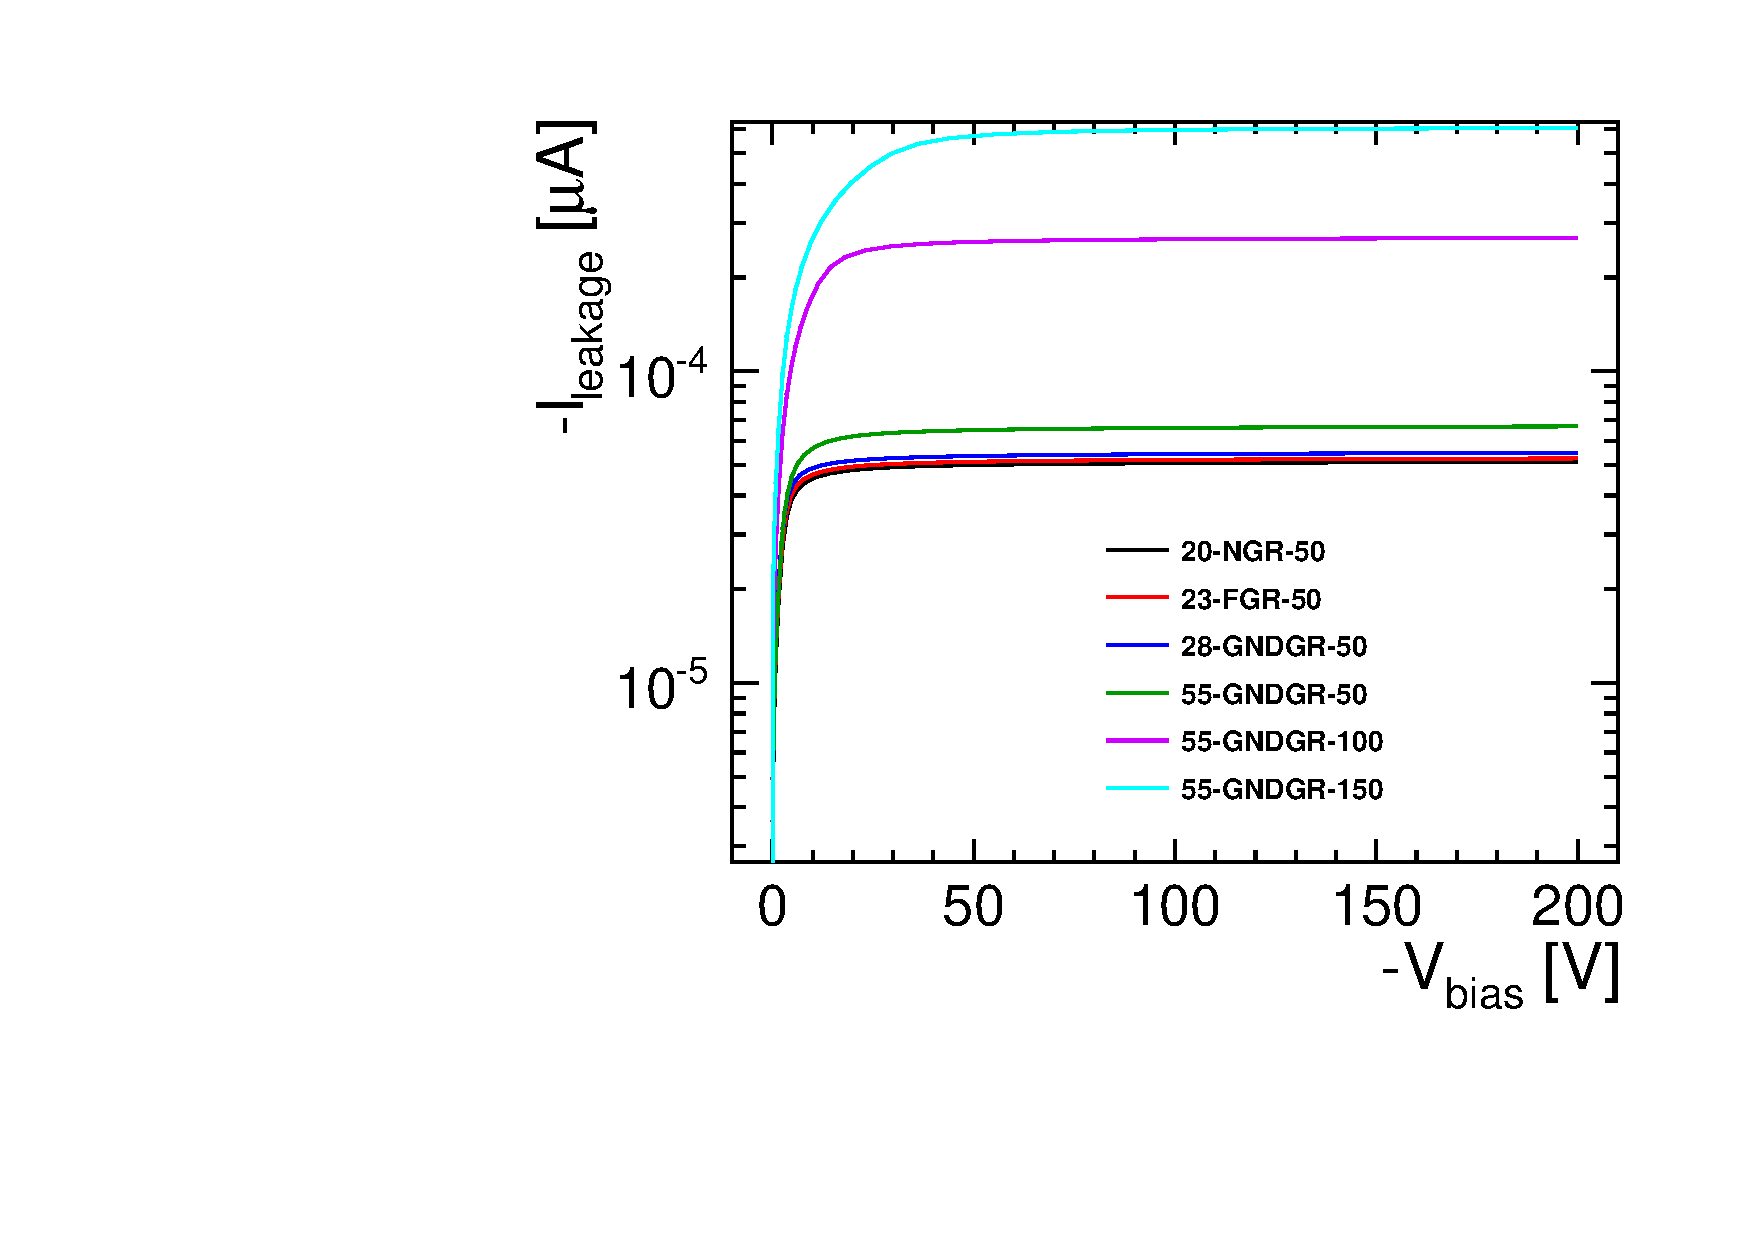
\includegraphics[width=\textwidth]{figures/ActiveEdge/IVCurve_TCAD.pdf}
    \caption{}
    \label{fig:IVmeasurements_TCAD}
  \end{subfigure}
  \caption{(a) Measured leakage current at the room temperature of
    $22^{\circ}$~C and (b) leakage current in TCAD simulations as a
    function of bias voltage for the active-edge assemblies listed in
    \cref{tab:Timepix3Assemblies}.}
  \label{fig:IVmeasurements_realANDtcad}
\end{figure}


%% --------------------------------------------- %%
%% \subsection{Electric field distribution in simulations}
%% \label{sec:TCAD_Efield_activeEdge}

In silicon, the breakdown occurs for electric fields exceeding
$\sim3\times10^5$~\voltpercm~\cite{Sze:100213}. In active-edge
sensors, since the back-side implantation as well as the bias voltage
are extended to the edge of the sensor, the gradient of potential
between the edge and the last pixel can be very high. This could lead
to a breakdown of the sensor. In TCAD simulations, the electric field
distribution for the sensors operated at nominal conditions are shown
in \cref{fig:TCAD_Efield2D}. In any case, for the nominal conditions
(c.f.~\cref{tab:nominalBiasThreshold}), the breakdown electric field
is never reached and in the laboratory measurements, this can be seen
through the measurement of the leakage current as shown in
\cref{fig:IVmeasurements}.

\begin{figure}[htbp]
  \centering
  \begin{subfigure}[b]{0.5\textwidth}
    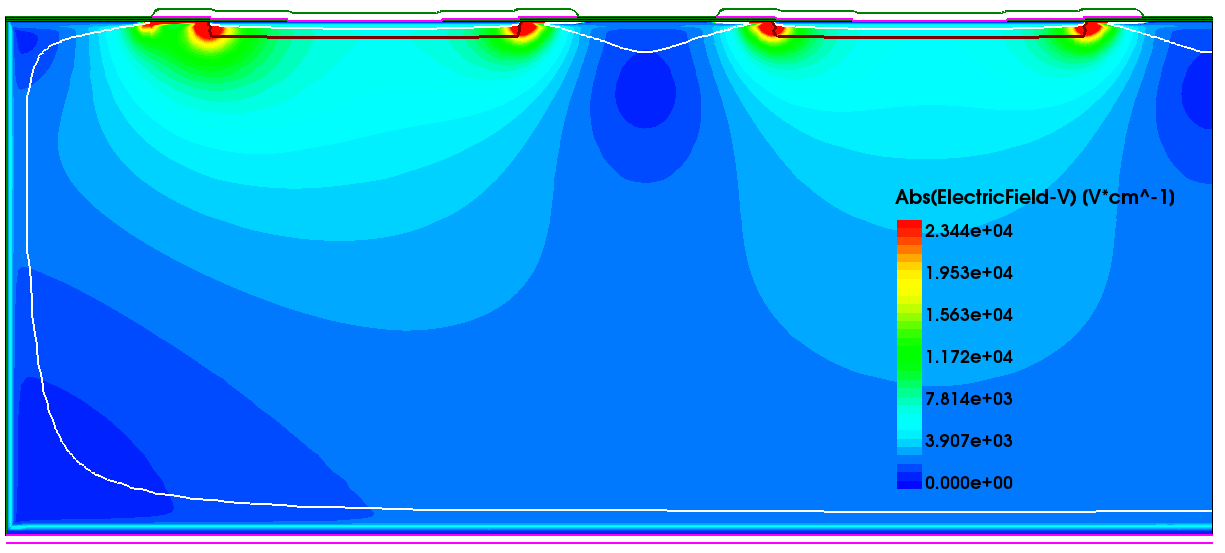
\includegraphics[width=\textwidth]{figures/ActiveEdge/Efield_20_NGR.png}
    \caption{20-NGR}
  \end{subfigure}\hfill
  \begin{subfigure}[b]{0.5\textwidth}
    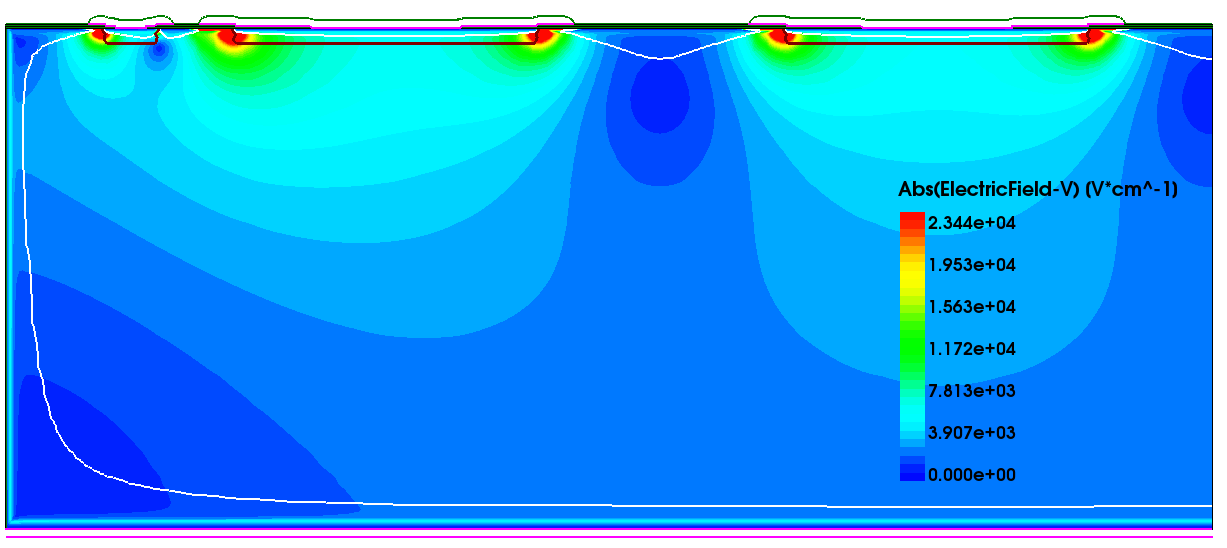
\includegraphics[width=\textwidth]{figures/ActiveEdge/Efield_23_FGR.png}
    \caption{23-FGR-50}
  \end{subfigure} \\
  \begin{subfigure}[b]{0.5\textwidth}
    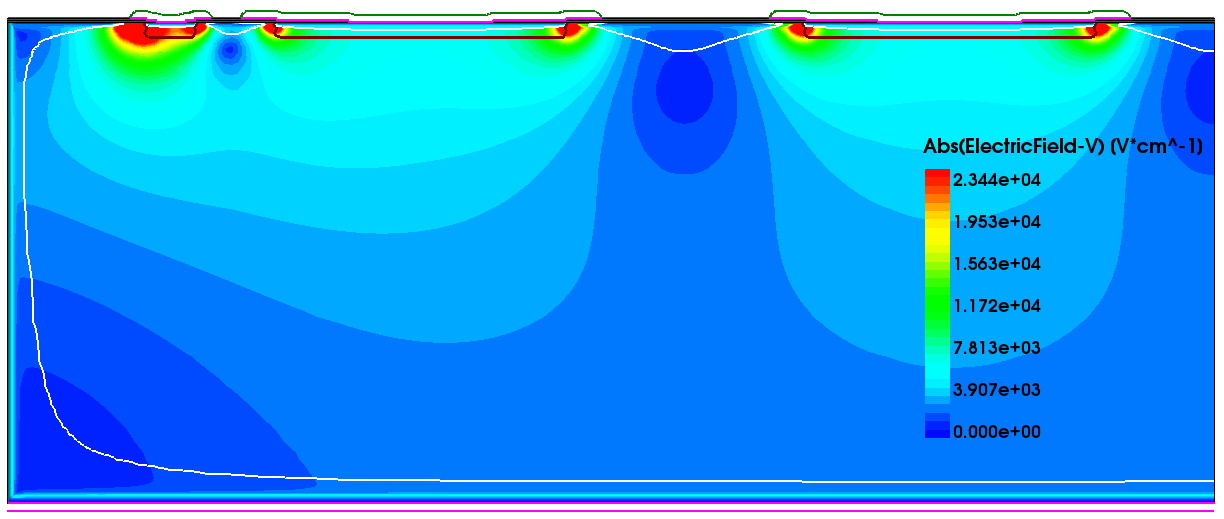
\includegraphics[width=\textwidth]{figures/ActiveEdge/Efield_28_GNDGR.png}
    \caption{28-GNDGR-50}
  \end{subfigure}\hfill
  \begin{subfigure}[b]{0.5\textwidth}
    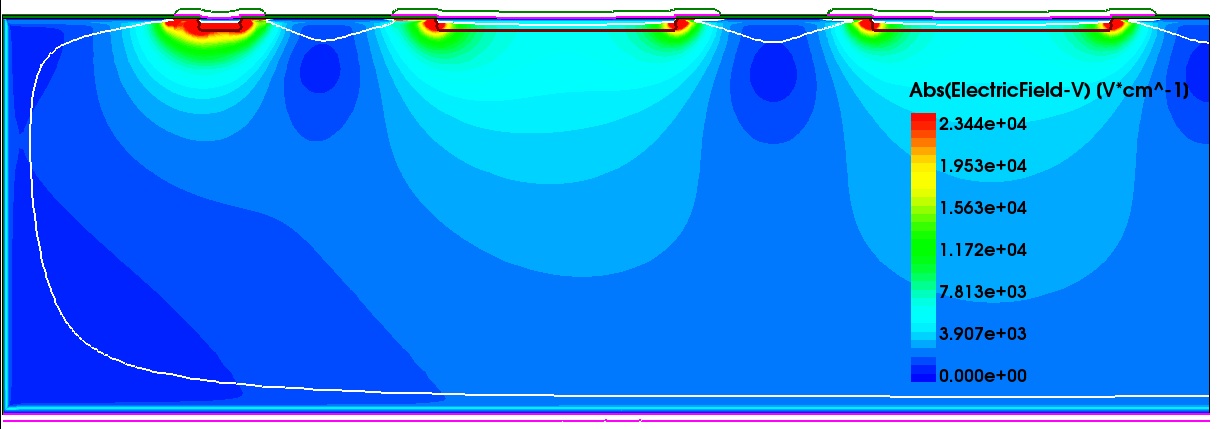
\includegraphics[width=\textwidth]{figures/ActiveEdge/Efield_55_GNDGR.png}
    \caption{55-GNDGR-50}
  \end{subfigure} \\
  \begin{subfigure}[b]{0.5\textwidth}
    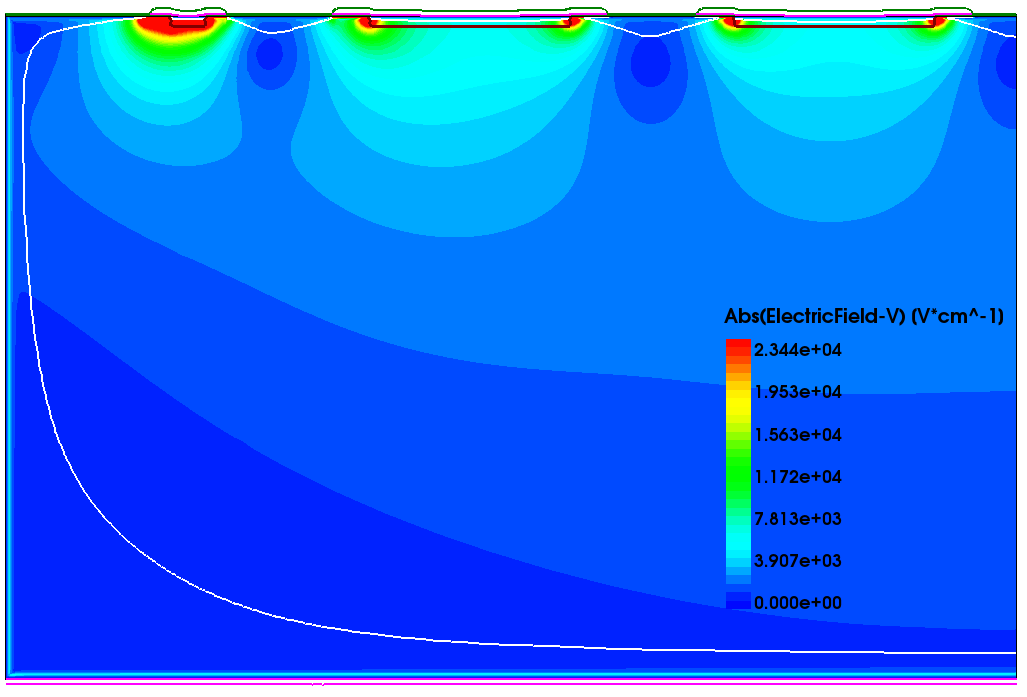
\includegraphics[width=\textwidth]{figures/ActiveEdge/Efield_55_GNDGR_100.png}
    \caption{55-GNDGR-100}
  \end{subfigure}\hfill
  \begin{subfigure}[b]{0.5\textwidth}
    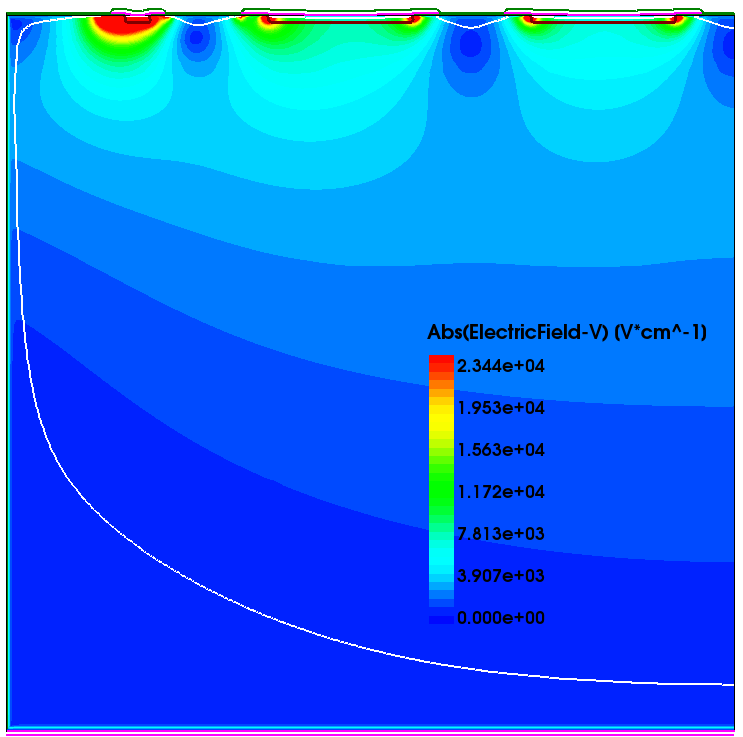
\includegraphics[width=\textwidth]{figures/ActiveEdge/Efield_55_GNDGR_150.png}
    \caption{55-GNDGR-150}
  \end{subfigure}
  \caption{Electric field distribution in TCAD simulations.}
  \label{fig:TCAD_Efield2D}
\end{figure}


The electric field and the electrostatic potential in TCAD simulations
for a cut close to the n-implants ($0.2\,\micron$ from the sensor
surface) are shown in
\cref{fig:TCAD_Efield_EPotential_sensorSurface}. Position $0\,\micron$
corresponds to the position of the first pixel. At the surface, the
breakdown electric field is never reached for the nominal
conditions. The floating guard-ring (23-FGR-50) results in a smoother
potential transition between the edge of the sensor and the first
pixel.


\begin{figure}[htbp]
  \centering
  \begin{subfigure}[b]{0.5\textwidth}
    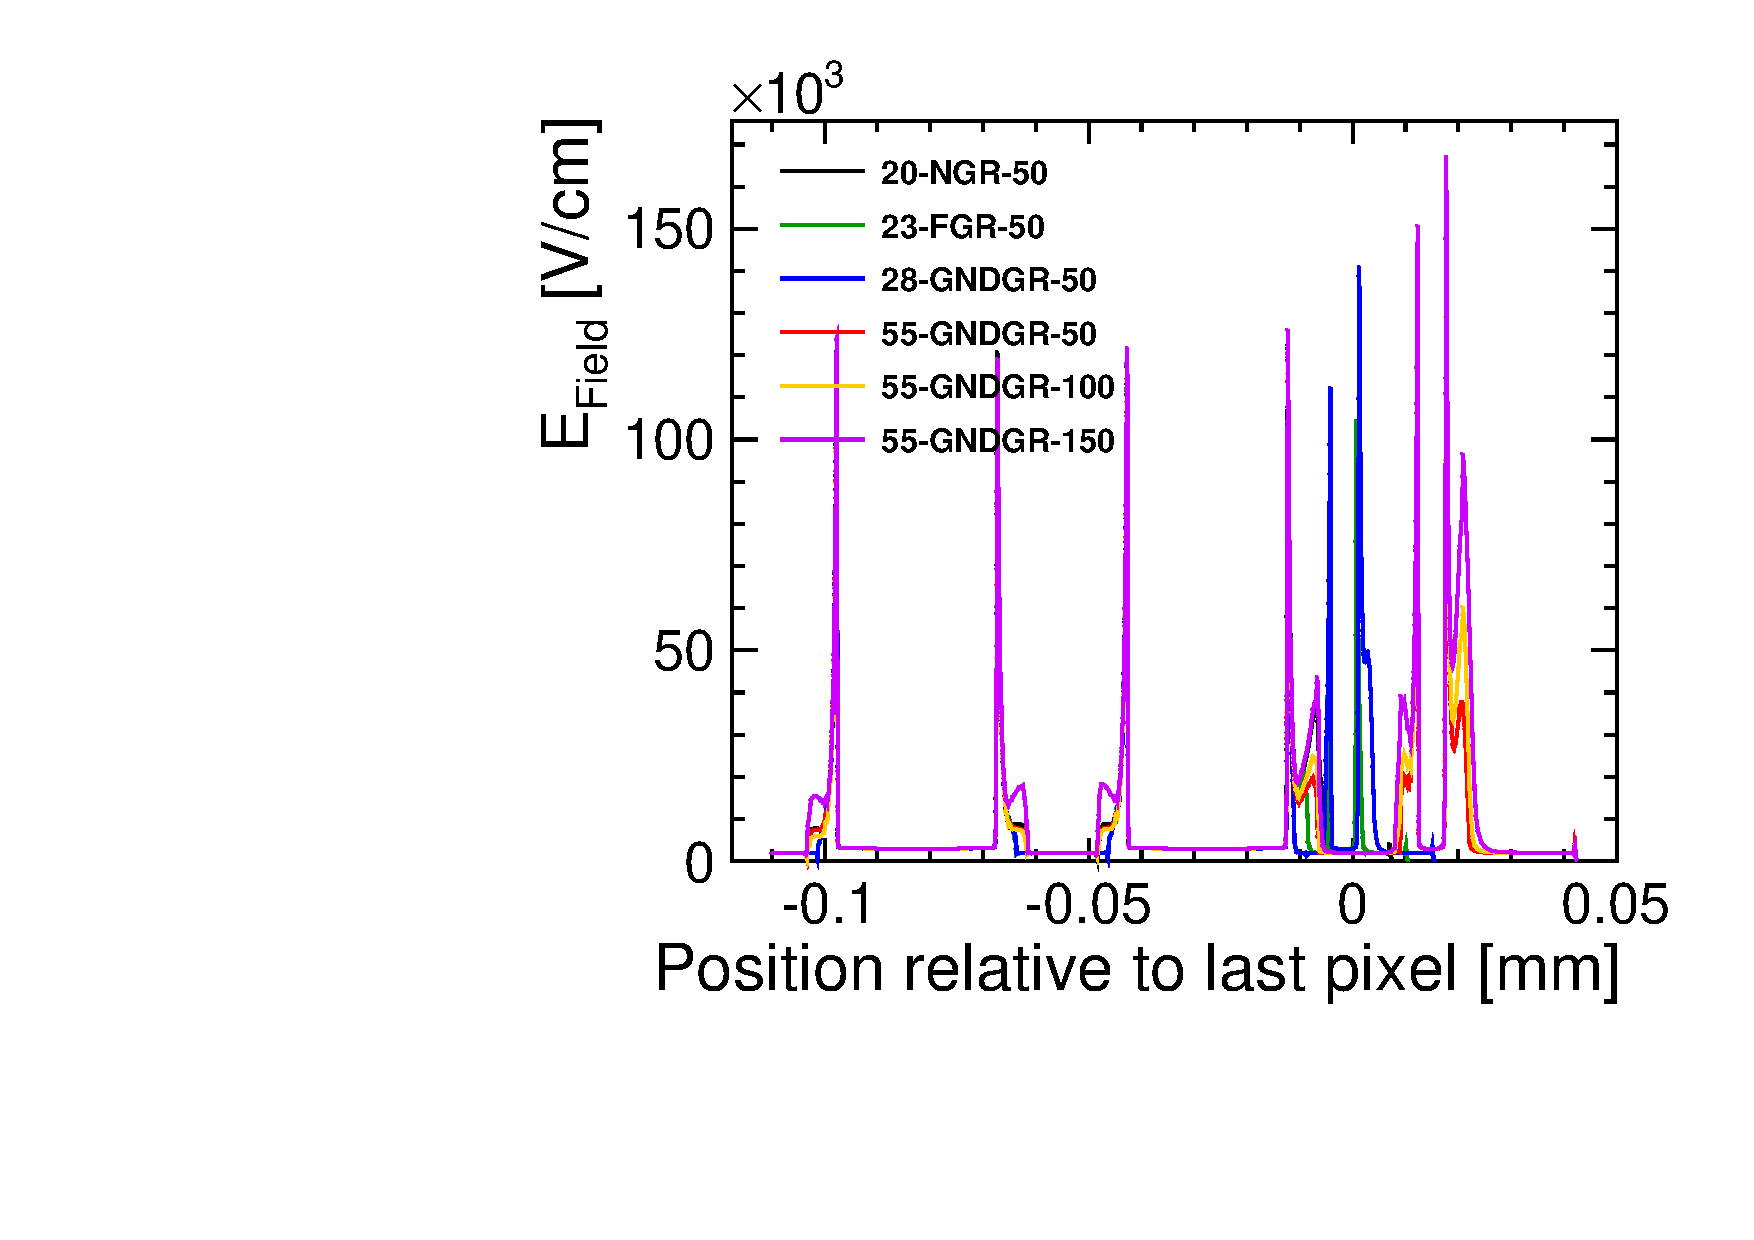
\includegraphics[width=\textwidth]{figures/ActiveEdge/Efiel_cut0_2um.pdf}
    \caption{}
  \end{subfigure}\hfill
  \begin{subfigure}[b]{0.5\textwidth}
    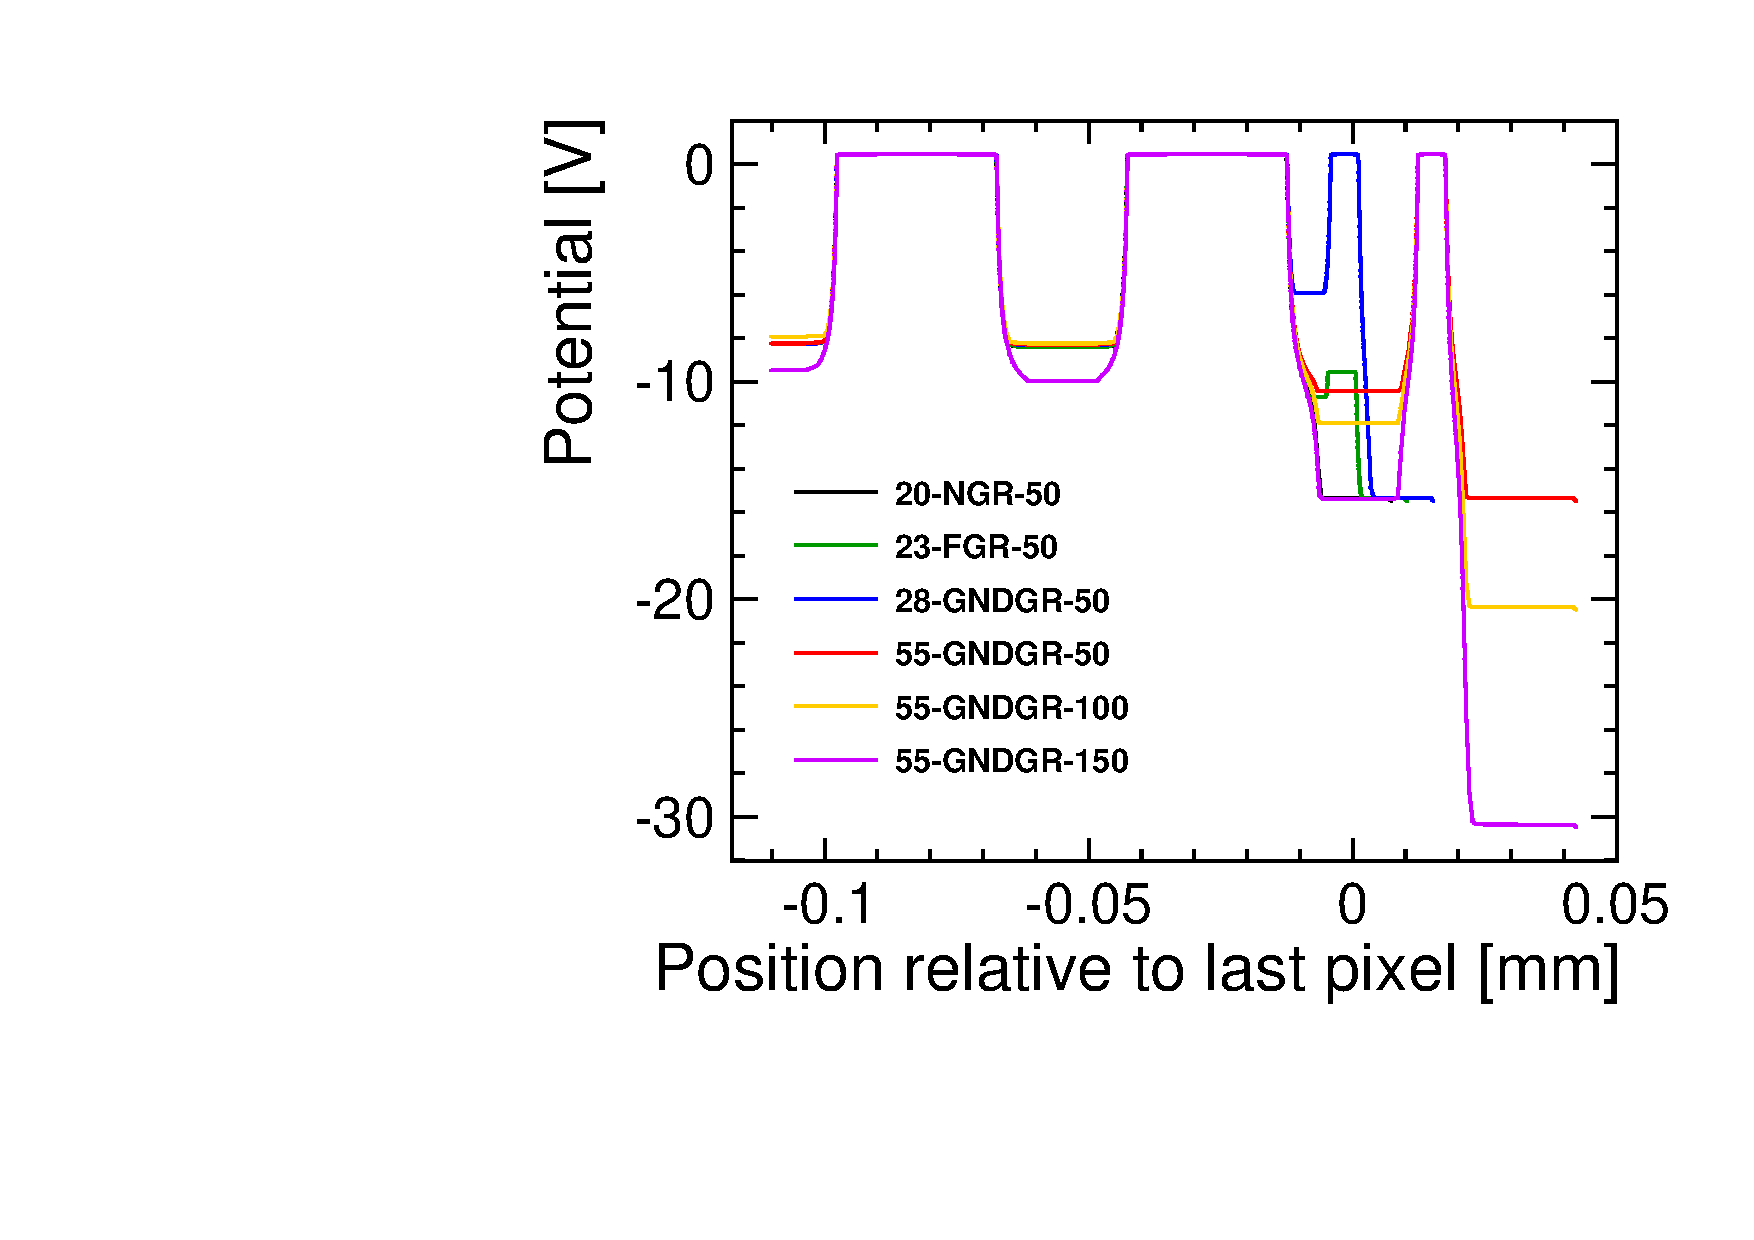
\includegraphics[width=\textwidth]{figures/ActiveEdge/EPotential_cut0_2um.pdf}
    \caption{}
  \end{subfigure}
  \caption{(a) The electric field and (b) the electrostatic potential
    for nominal bias voltage at a distance of $0.2\,\micron$ from the
    sensor surface. Position $0\,\micron$ corresponds to the position
    of the first pixel.}
  \label{fig:TCAD_Efield_EPotential_sensorSurface}
\end{figure}

%% --------------------------------------------- %%
\newpage
\section{Edge performance in data and simulations}
The active-edge assemblies are tested at the CERN SPS with $120\,\gev$
pions (c.f. \cref{sec:CERN_SPS}), making use of the Timepix3 beam
reference telescope as described in \cref{ch:Telescope}. The edge
performance is investigated in terms of the efficiency of detecting a
track and the amount of collected charge as a function of the track
position on the edge.

%% --------------------------------------------- %%
\subsection{TCAD simulation of the detector response}
\label{sec:TCAD_Simu_ActiveEdge}

TCAD simulations are used to study the charge collection in the edge
region. The process flow as described in \cref{sec:processFlowTCAD} is
used to simulate two pixels and the edge region in a 2D
configuration. The transient simulation of the active edge devices is
done by a charge deposition of $10^{-5}\,\picocoulomb/\micron$ along
the particle track. This corresponds to an energy deposition of
$\sim80\,\text{e-}/\micron$ as expected for the MIP in
silicon. \cref{fig:TCAD_transientSimu} illustrates an example of a MIP
traversing the sensor at a distance of $10\,\micron$ from the left
edge 6~ns after the particle hit. The electron density is shown in
this figure. 

In simulation, hits are generated at different positions. The
electrodes collect the signal created by the electrons since the
sensor is of type n-in-p. The signal is integrated over 15~ns. The
peaking time of the signal is usually less than 5~ns therefore the
integration time is enough to collect most of the signal.

\begin{figure}[htbp]
  \centering
  \begin{tikzpicture}
    \node[anchor=south west,inner sep=0] (image) at
    (0,0){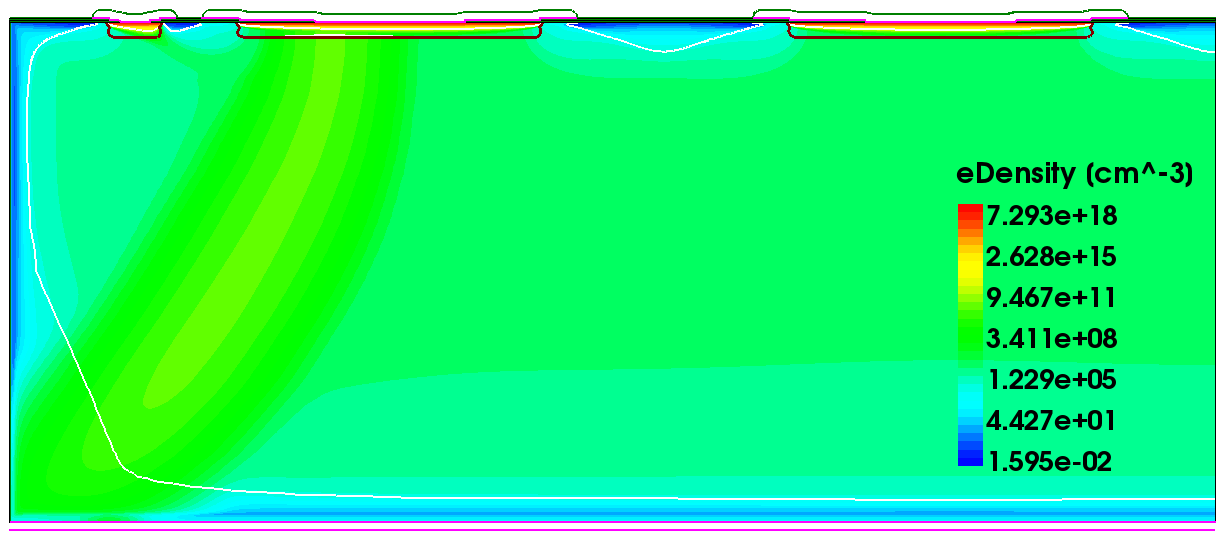
\includegraphics[width=0.7\textwidth]{figures/ActiveEdge/TCAD_transient_23FGR_hitpos_60.png}};
    \begin{scope}[x={(image.south east)},y={(image.north west)}]

      %% \draw[help lines,xstep=.1,ystep=.1] (0, 0) grid (1,1);
      %% \foreach \x in {0,1,...,9} { \node [anchor=north] at (\x/10,0) {0.\x}; }
      %% \foreach \y in {0,1,...,9} { \node [anchor=east] at (0,\y/10) {0.\y}; }

      \draw[->, very thick] (0.093, 0.0) -- (0.093, 1.05);
    \end{scope}
  \end{tikzpicture}
  \caption{Transient simulation of a particle track traversing the
    sensor at a distance of $10\,\micron$ from the edge (illustrated
    as an arrow). The electron density 6~ns after the particle hit is
    shown. The region shown with a white line is the depletion
    region.}
  \label{fig:TCAD_transientSimu}
\end{figure}



%% --------------------------------------------- %%
\newpage
\subsection{Results}
\label{sec:activeEdge_results}

The performance of the edge is studied in data in terms of the
efficiency and the collected charge at the edge as a function of the
track position. The collected charge at the edge is also simulated (as
described in \cref{sec:TCAD_Simu_ActiveEdge}) and compared to the
data. The convention as illustrated in \cref{fig:Layout20_NGR} is used
to show the performance of the different assemblies in
\cref{fig:20-NGR_eff_TOT,fig:23-FGR_eff_TOT,fig:28-GNDGR_eff_TOT,fig:55-GNDGR_eff_TOT,fig:55-GNDGR-100_eff_TOT,fig:55-GNDGR-150_eff_TOT}. The
border of the last pixel (at 0~mm) is indicated with a dashed line and
the physical sensor edge is shown as a continuous line. The detection
efficiency is calculated by counting the number of tracks matched to
hits on the DUT divided by the total number of tracks projected on the
DUT. The efficiency within the pixels is then mapped into a grid of
$2\times2$ pixels. The x-axis shows the track position relative to the
last pixel. The y-axis combines the tracks for the even rows (in the
coordinates between 0~mm and 0.055~mm) and the odd rows (in the
coordinates between 0.055~mm and 0.11~mm). The z-axis shows the
efficiency for the plots on the left. To increase the statistics, the
beam was focused on only one of the edges during the data taking.

The assemblies without (\cref{fig:20-NGR_eff_TOT}) and with floating
guard ring (\cref{fig:23-FGR_eff_TOT}) are efficient up to the
physical edge of the sensor. The charge is fully collected by the last
pixel for 20-NGR-50. For 23-FGR-50, a loss of the charge near the edge
is observed (charge lost in the guard ring).

\begin{figure}[htbp]
  \begin{subfigure}[b]{0.5\textwidth}
    \centering
    \begin{tikzpicture}
      \node[anchor=south west,inner sep=0] (image) at (0,0) {
        \includegraphics[width=\textwidth, page=3]{figures/TestBeam/edge_bcp.pdf}};
    \end{tikzpicture}
    \caption{}
  \end{subfigure}\hfill
  \begin{subfigure}[b]{0.5\textwidth}
    \centering
    \begin{tikzpicture}
      \node[anchor=south west,inner sep=0] (image) at 
      (0,0){\includegraphics[width=\textwidth, page=5]{figures/TestBeam/edge.pdf}};
    \end{tikzpicture}
    \caption{}
  \end{subfigure}
  \caption{(a) Efficiency and (b) charge (TOT) collected as a function of the
    track position for the assembly 20-NGR-50.}
  \label{fig:20-NGR_eff_TOT}
\end{figure}


\begin{figure}[htbp]
  \begin{subfigure}[b]{0.5\textwidth}
    \centering
    \begin{tikzpicture}
      \node[anchor=south west,inner sep=0] (image) at (0,0)
      {\includegraphics[width=\textwidth, page=6]{figures/TestBeam/edge_bcp.pdf}};
    \end{tikzpicture}
    \caption{}
  \end{subfigure}\hfill
  \begin{subfigure}[b]{0.5\textwidth}
    \centering
    \begin{tikzpicture}
      \node[anchor=south west,inner sep=0] (image) at 
      (0,0){\includegraphics[width=\textwidth, page=8]{figures/TestBeam/edge.pdf}};
    \end{tikzpicture}
    \caption{}
  \end{subfigure}
  \caption{(a) Efficiency and (b) charge (TOT) collected as a function of the
    track position for the assembly 23-FGR-50.}
  \label{fig:23-FGR_eff_TOT}
\end{figure}

The grounded guard ring degrades significantly the detection
efficiency at the edge. For 28-GNDGR-50, the efficiency drops between
pixels as shown in \cref{fig:28-GNDGR_eff_TOT}. A large part of the
charge is collected by the guard ring. For 55-GNDGR-50, as shown in
\cref{fig:55-GNDGR_eff_TOT}, the edge is not efficient anymore due to
the reduced amount of detected charge in thin sensors and its low
sharing to the neighbouring pixels (lower than the threshold of the
readout chip). All of the charge created in the edge is collected by
the guard ring.

\begin{figure}[htbp]
  \begin{subfigure}[b]{0.5\textwidth}
    \centering
    \begin{tikzpicture}
      \node[anchor=south west,inner sep=0] (image) at (0,0)
      {\includegraphics[width=\textwidth, page=9]{figures/TestBeam/edge_bcp.pdf}};
    \end{tikzpicture}
    \caption{}
  \end{subfigure}~
  \begin{subfigure}[b]{0.5\textwidth}
    \centering
    \begin{tikzpicture}
      \node[anchor=south west,inner sep=0] (image) at 
      (0,0){\includegraphics[width=\textwidth, page=11]{figures/TestBeam/edge.pdf}};
    \end{tikzpicture}
    \caption{}
  \end{subfigure}
  \caption{(a) Efficiency and (b) charge (TOT) collected as a function of the
    track position for the assembly 28-GNDGR-50.}
  \label{fig:28-GNDGR_eff_TOT}
\end{figure}


\begin{figure}[htbp]
  \begin{subfigure}[b]{0.5\textwidth}
    \centering
    \begin{tikzpicture}
      \node[anchor=south west,inner sep=0] (image) at (0,0)
      {\includegraphics[width=\textwidth, page=12]{figures/TestBeam/edge_bcp.pdf}};
    \end{tikzpicture}
    \caption{}
  \end{subfigure}\hfill
  \begin{subfigure}[b]{0.5\textwidth}
    \centering
    \begin{tikzpicture}
      \node[anchor=south west,inner sep=0] (image) at 
      (0,0){\includegraphics[width=\textwidth,
        page=14]{figures/TestBeam/edge.pdf}};
    \end{tikzpicture}
    \caption{}
  \end{subfigure}
  \caption{(a) Efficiency and (b) charge (TOT) collected as a function
    of the track position for the assembly 55-GNDGR-50.}
  \label{fig:55-GNDGR_eff_TOT}
\end{figure}

For thin sensors, a floating guard ring appears to be the most
suitable solution, as it shows a high detection efficiency at the edge
and an acceptable breakdown behaviour
(\cref{fig:IVmeasurements}). Tests with additional assemblies will be
needed to confirm this observation.

For the thicker sensors ($100\,\micron$ and $150\,\micron$), the
grounded guard ring is a suitable solution. The assemblies
55-GNDGR-100 and 55-GNDGR-150 are efficient up to the edge even with a
loss of the charge near the edge as shown in
\cref{fig:55-GNDGR-100_eff_TOT,fig:55-GNDGR-150_eff_TOT}.

\begin{figure}[htbp]
  \begin{subfigure}[b]{0.5\textwidth}
    \centering
    \begin{tikzpicture}
      \node[anchor=south west,inner sep=0] (image) at (0,0)
      {\includegraphics[width=\textwidth, page=15]{figures/TestBeam/edge_bcp.pdf}};
    \end{tikzpicture}
    \caption{}
  \end{subfigure}\hfill
  \begin{subfigure}[b]{0.5\textwidth}
    \centering
    \begin{tikzpicture}
      \node[anchor=south west,inner sep=0] (image) at 
      (0,0){\includegraphics[width=\textwidth,
        page=17]{figures/TestBeam/edge.pdf}};
    \end{tikzpicture}
    \caption{}
  \end{subfigure}
  \caption{(a) Efficiency and (b) charge (TOT) collected as a function of the
    track position for the assembly 55-GNDGR-100.}
  \label{fig:55-GNDGR-100_eff_TOT}
\end{figure}


\begin{figure}[htbp]
  \begin{subfigure}[b]{0.5\textwidth}
    \centering
    \begin{tikzpicture}
      \node[anchor=south west,inner sep=0] (image) at (0,0)
      {\includegraphics[width=\textwidth, page=18]{figures/TestBeam/edge_bcp.pdf}};
    \end{tikzpicture}
    \caption{}
  \end{subfigure}\hfill
  \begin{subfigure}[b]{0.5\textwidth}
    \centering
    \begin{tikzpicture}
      \node[anchor=south west,inner sep=0] (image) at 
      (0,0){\includegraphics[width=\textwidth,
        page=20]{figures/TestBeam/edge.pdf}};
    \end{tikzpicture}
    \caption{}
  \end{subfigure}
  \caption{(a) Efficiency and (b) charge (TOT) collected as a function of the
    track position for the assembly 55-GNDGR-150.}
  \label{fig:55-GNDGR-150_eff_TOT}
\end{figure}

\cref{fig:EdgeEff_2D} summarises the edge efficiency as a function of
the track position relative to the edge projected in one direction for
the different assemblies.

\begin{figure}[htbp]
  \centering
  %EdgeEfficiency_2D.py
  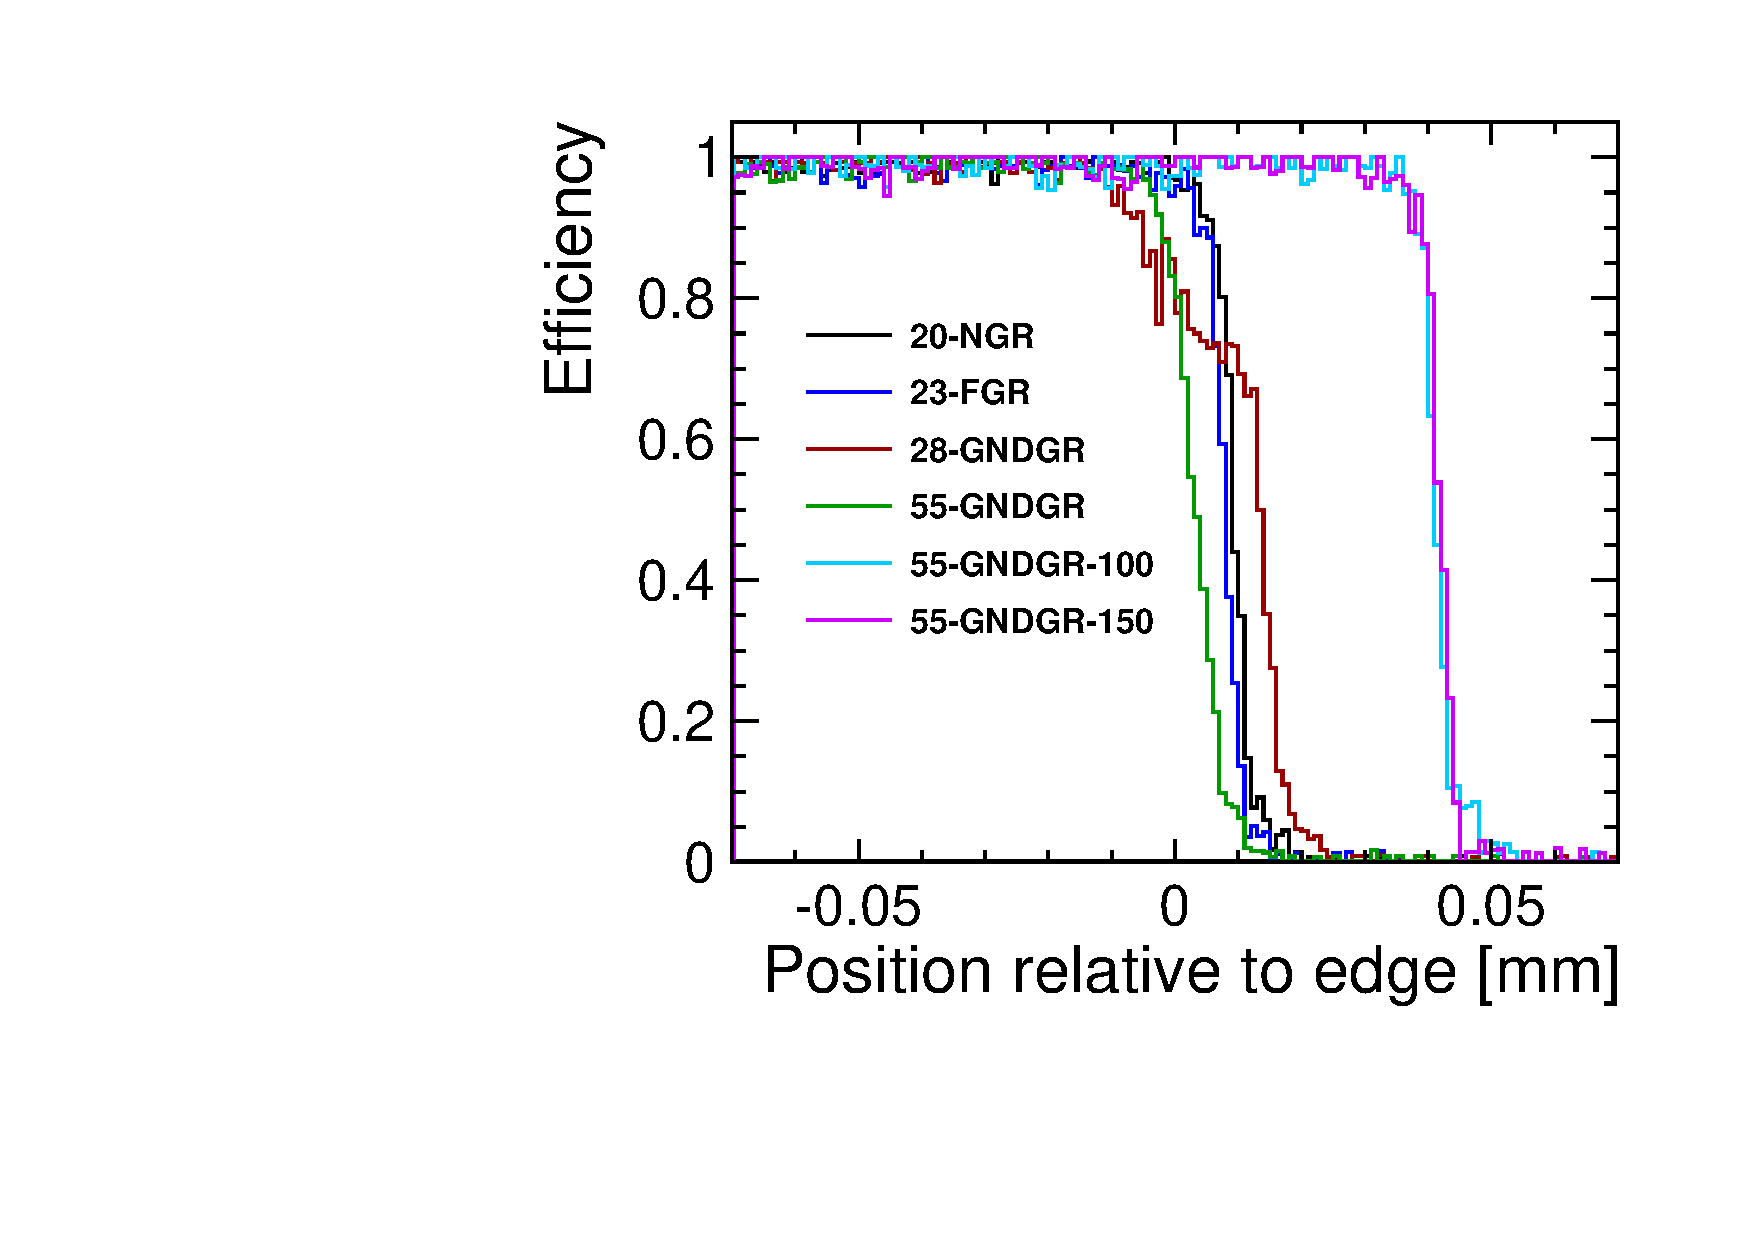
\includegraphics[width=0.7\textwidth]{figures/ActiveEdge/edgeEff_2D.pdf}
  \caption{The edge efficiency as a function of the track position
    relative to the edge projected in one direction.}
  \label{fig:EdgeEff_2D}
\end{figure}

%% %% --------------------------------------------- %%
%% \newpage
%% \section{TCAD simulations of active-edge sensors}





%% --------------------------------------------- %%
%% \subsection{Validation of simulation with
%%   data}\label{sec:TCAD_dataValidation_activeEdge}

%% The transient simulation of the active edge devices is done by a
%% charge deposition of $10^{-5}\,\picocoulomb/\micron$ along the
%% particle track. This corresponds to an energy deposition of
%% $\sim80\,\text{e-}/\micron$ as expected for the MIP in
%% silicon. \cref{fig:TCAD_transientSimu} illustrates a MIP traversing
%% the sensor at a distance of $10\,\micron$ from the left edge. The
%% electron density 6~ns after the particle hit is illustrated. The
%% electrodes collect the current generated by the electrons and it is
%% integrated over 15~ns.

%% \begin{figure}[htbp]
%%   \centering
%%   \begin{tikzpicture}
%%     \node[anchor=south west,inner sep=0] (image) at
%%     (0,0){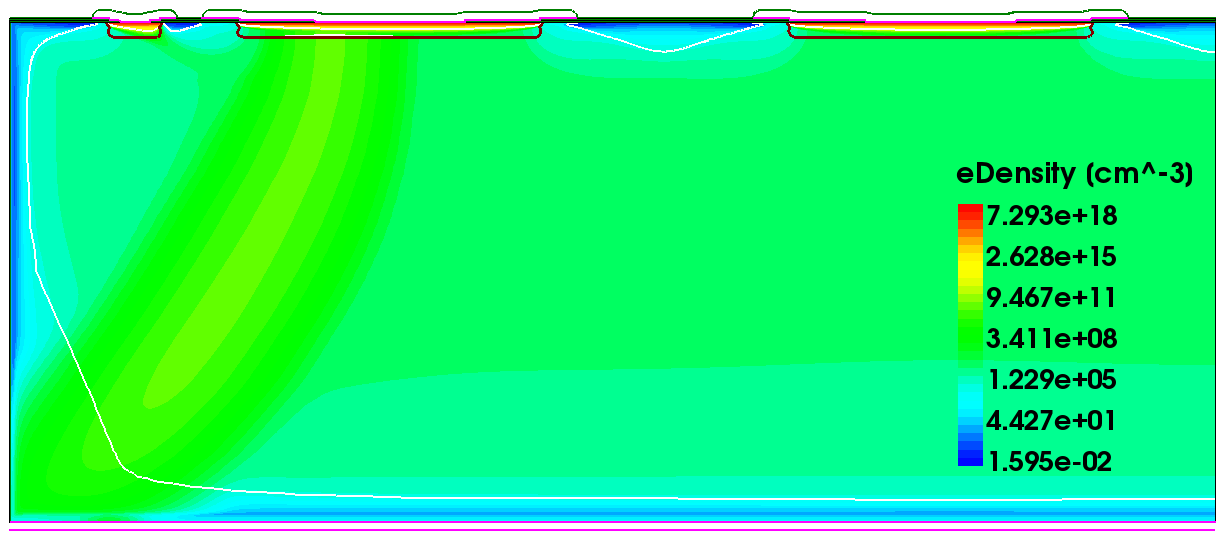
\includegraphics[width=0.7\textwidth]{figures/ActiveEdge/TCAD_transient_23FGR_hitpos_60.png}};
%%     \begin{scope}[x={(image.south east)},y={(image.north west)}]

%%       %% \draw[help lines,xstep=.1,ystep=.1] (0, 0) grid (1,1);
%%       %% \foreach \x in {0,1,...,9} { \node [anchor=north] at (\x/10,0) {0.\x}; }
%%       %% \foreach \y in {0,1,...,9} { \node [anchor=east] at (0,\y/10) {0.\y}; }

%%       \draw[->, very thick] (0.093, 0.0) -- (0.093, 1.05);
%%     \end{scope}
%%   \end{tikzpicture}
%%   \caption{Transient simulation of a particle track traversing the
%%     sensor at a distance of $10\,\micron$ from the edge (the
%%     arrow). The electron density 6~ns after the particle hit is
%%     shown.}
%%   \label{fig:TCAD_transientSimu}
%% \end{figure}


%% In simulation, hits are generated at different positions. The charge
%% collected by each electrode is calculated over the integration
%% time. 
\cref{fig:TCAD_vs_data_20_NGR,fig:TCAD_vs_data_23_FGR,fig:TCAD_vs_data_28_GNDGR,fig:TCAD_vs_data_55_GNDGR,fig:TCAD_vs_data_55_GNDGR_100,fig:TCAD_vs_data_55_GNDGR_150}
compare the charge collected as a function of the hit position in data
and TCAD simulations. In data, the charge deposited is plotted versus
the track position given by the Timepix3 telescope (with a resolution
of $\sim2\,\micron$). The charge deposited is obtained by applying the
test-pulse calibrations to the data. For each track position, the
deposited charge is projected as a one-dimensional histogram and
fitted with a Landau function convoluted with a Gaussian. The most
probable value (MPV) of the Landau fit is then compared to the
collected charge obtained in the TCAD simulations. In the TCAD
simulations, a fixed amount of charge is deposited and, unlike the
data, the fluctuations of the deposited charge are not
considered. This can explain the minor discrepancies on the amount of
the collected charge between simulation and data. The border of the
last pixel (at 0~mm) is indicated with a dashed line and the physical
sensor edge is shown in continuous line with the convention as
illustrated in \cref{fig:Layout20_NGR}.

For 20-NGR, the TCAD simulation agrees well with the data observation
as shown in \cref{fig:TCAD_vs_data_20_NGR}.

\begin{figure}[htbp]
  \centering
  \begin{subfigure}[b]{0.5\textwidth}
    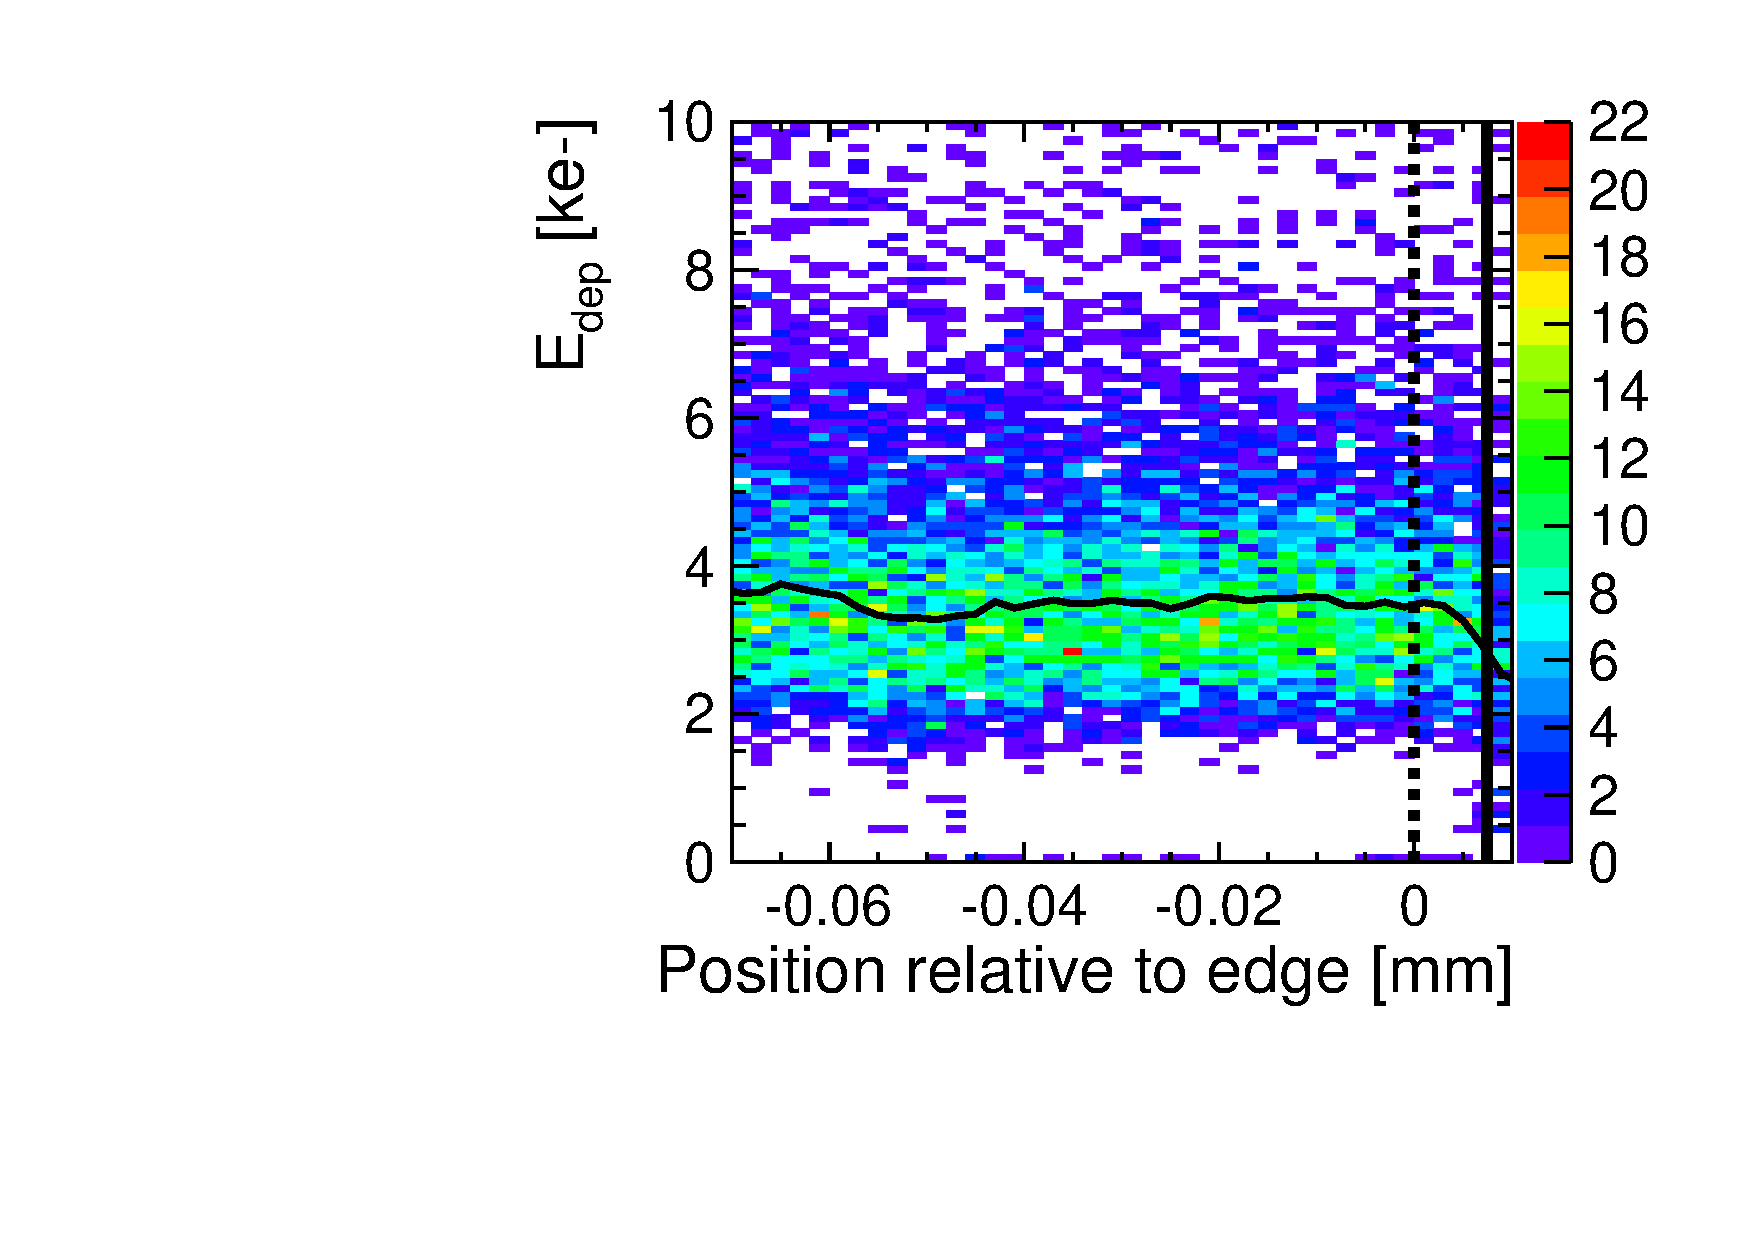
\includegraphics[width=\textwidth]{figures/ActiveEdge/TCAD_data_Edep_20_NGR.pdf}
    \caption{}
  \end{subfigure}\hfill
  \begin{subfigure}[b]{0.5\textwidth}
    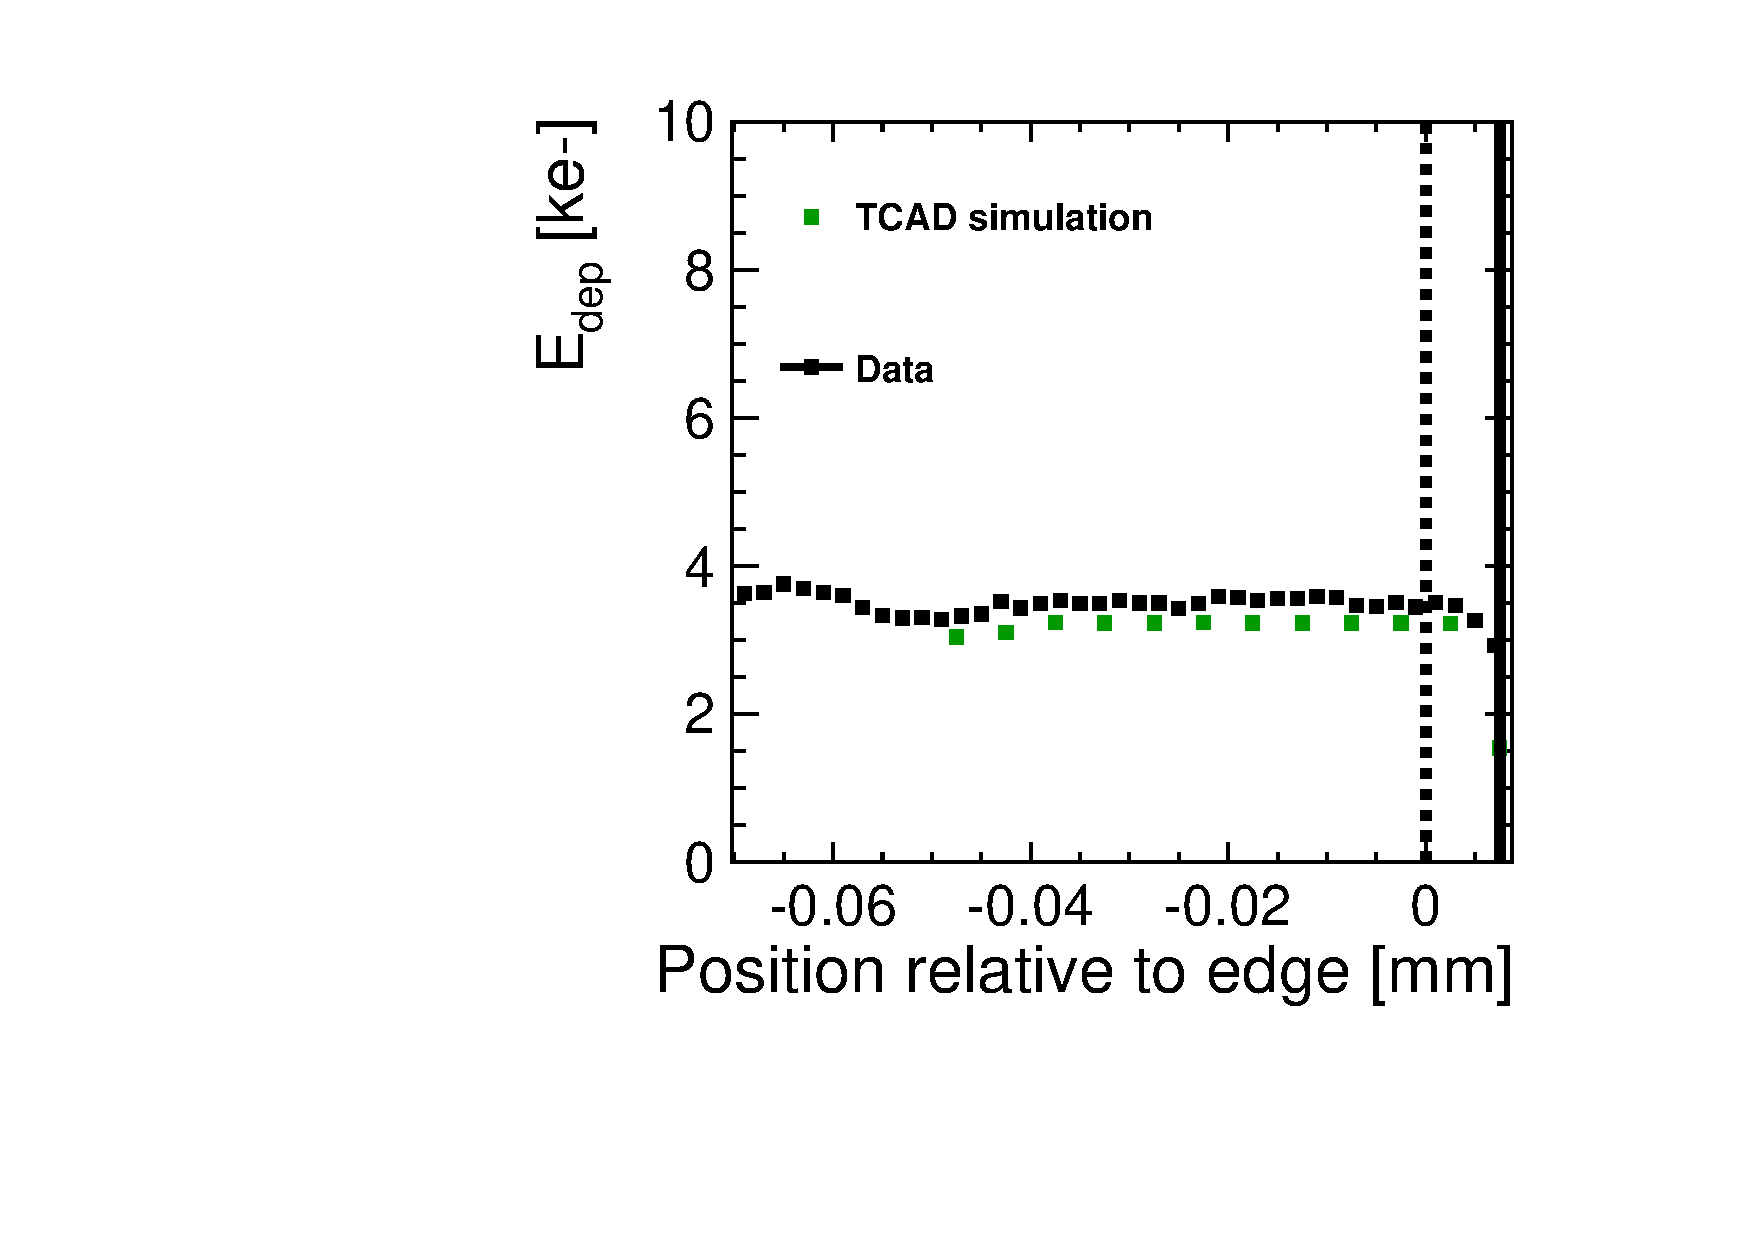
\includegraphics[width=\textwidth]{figures/ActiveEdge/TCAD_data_20_NGR.pdf}
    \caption{}
  \end{subfigure}
  \caption{20-NGR}
  \label{fig:TCAD_vs_data_20_NGR}
\end{figure}

To simulate a floating guard ring for 23-FGR, in TCAD, the electrode
on the guard ring is forced to have no current and the potential is
left undefined. The agreement seems good but in data it seems that
more charge is collected by the guard ring than in simulation as shown
in \cref{fig:TCAD_vs_data_23_FGR}.
 
\begin{figure}[htbp]
  \centering
  \begin{subfigure}[b]{0.5\textwidth}

    \caption{}
  \end{subfigure}\hfill
  \begin{subfigure}[b]{0.5\textwidth}
    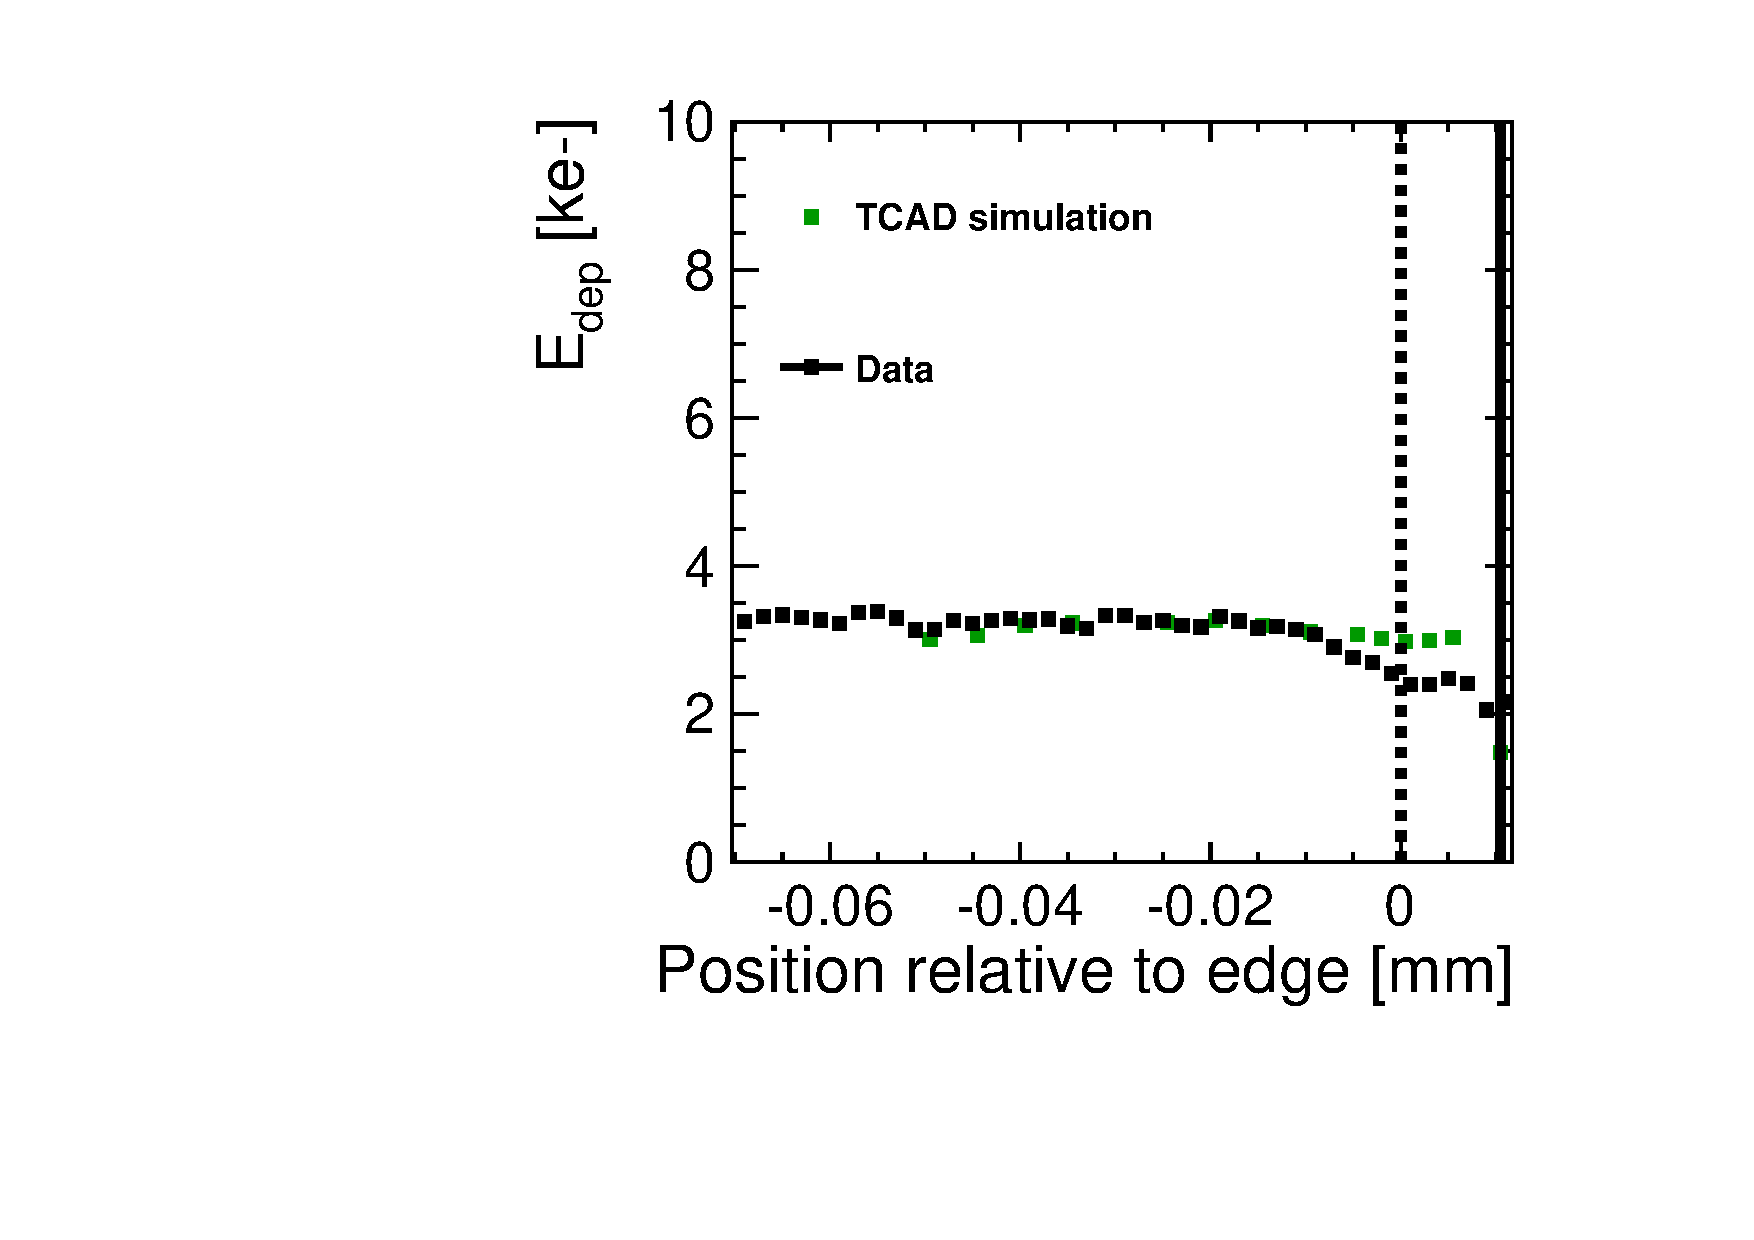
\includegraphics[width=\textwidth]{figures/ActiveEdge/TCAD_data_23_FGR.pdf}
    \caption{}
  \end{subfigure}
  \caption{23-FGR: no calibration is available: TOT is multiplied by 128 to obtain the Edep in electrons.}
  \label{fig:TCAD_vs_data_23_FGR}
\end{figure}

In the TCAD simulations for the grounded guard ring configurations,
the electrode of the guard ring is forced to have no current and the
potential is forced to be 0~V. For 28-GNDGR and 55-GNDGR, the TCAD
simulations show a drop in the collected charge but less than in data
as shown in
\cref{fig:TCAD_vs_data_28_GNDGR,fig:TCAD_vs_data_55_GNDGR}. For
55-GNDGR, in TCAD simulations charges are collected by the pixel even
for hit positions which are very close to the physical edge since no
threshold was applied in simulation. In data a threshold of $\sim$500
electrons is applied.

\begin{figure}[htbp]
  \centering
  \begin{subfigure}[b]{0.5\textwidth}
    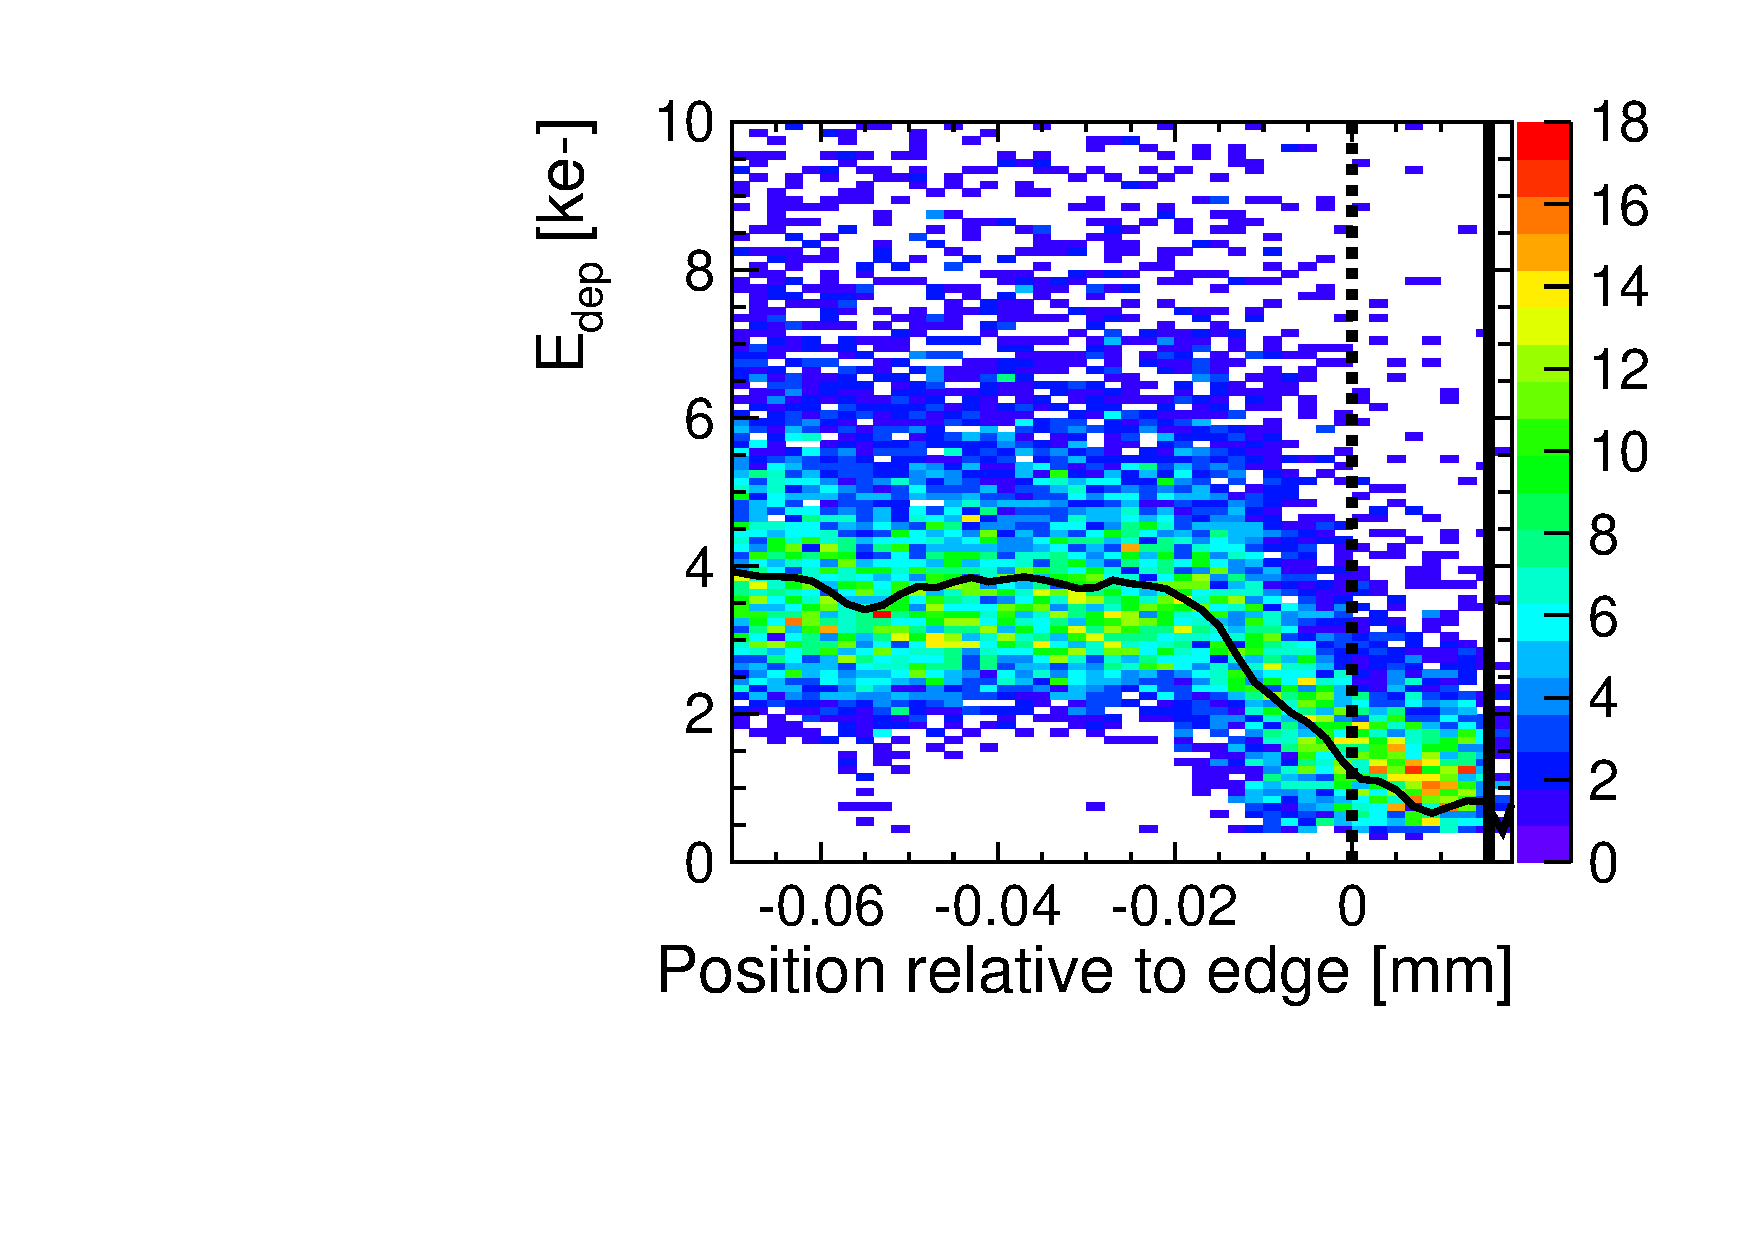
\includegraphics[width=\textwidth]{figures/ActiveEdge/TCAD_data_Edep_28_GNDGR.pdf}
    \caption{}
  \end{subfigure}\hfill
  \begin{subfigure}[b]{0.5\textwidth}
    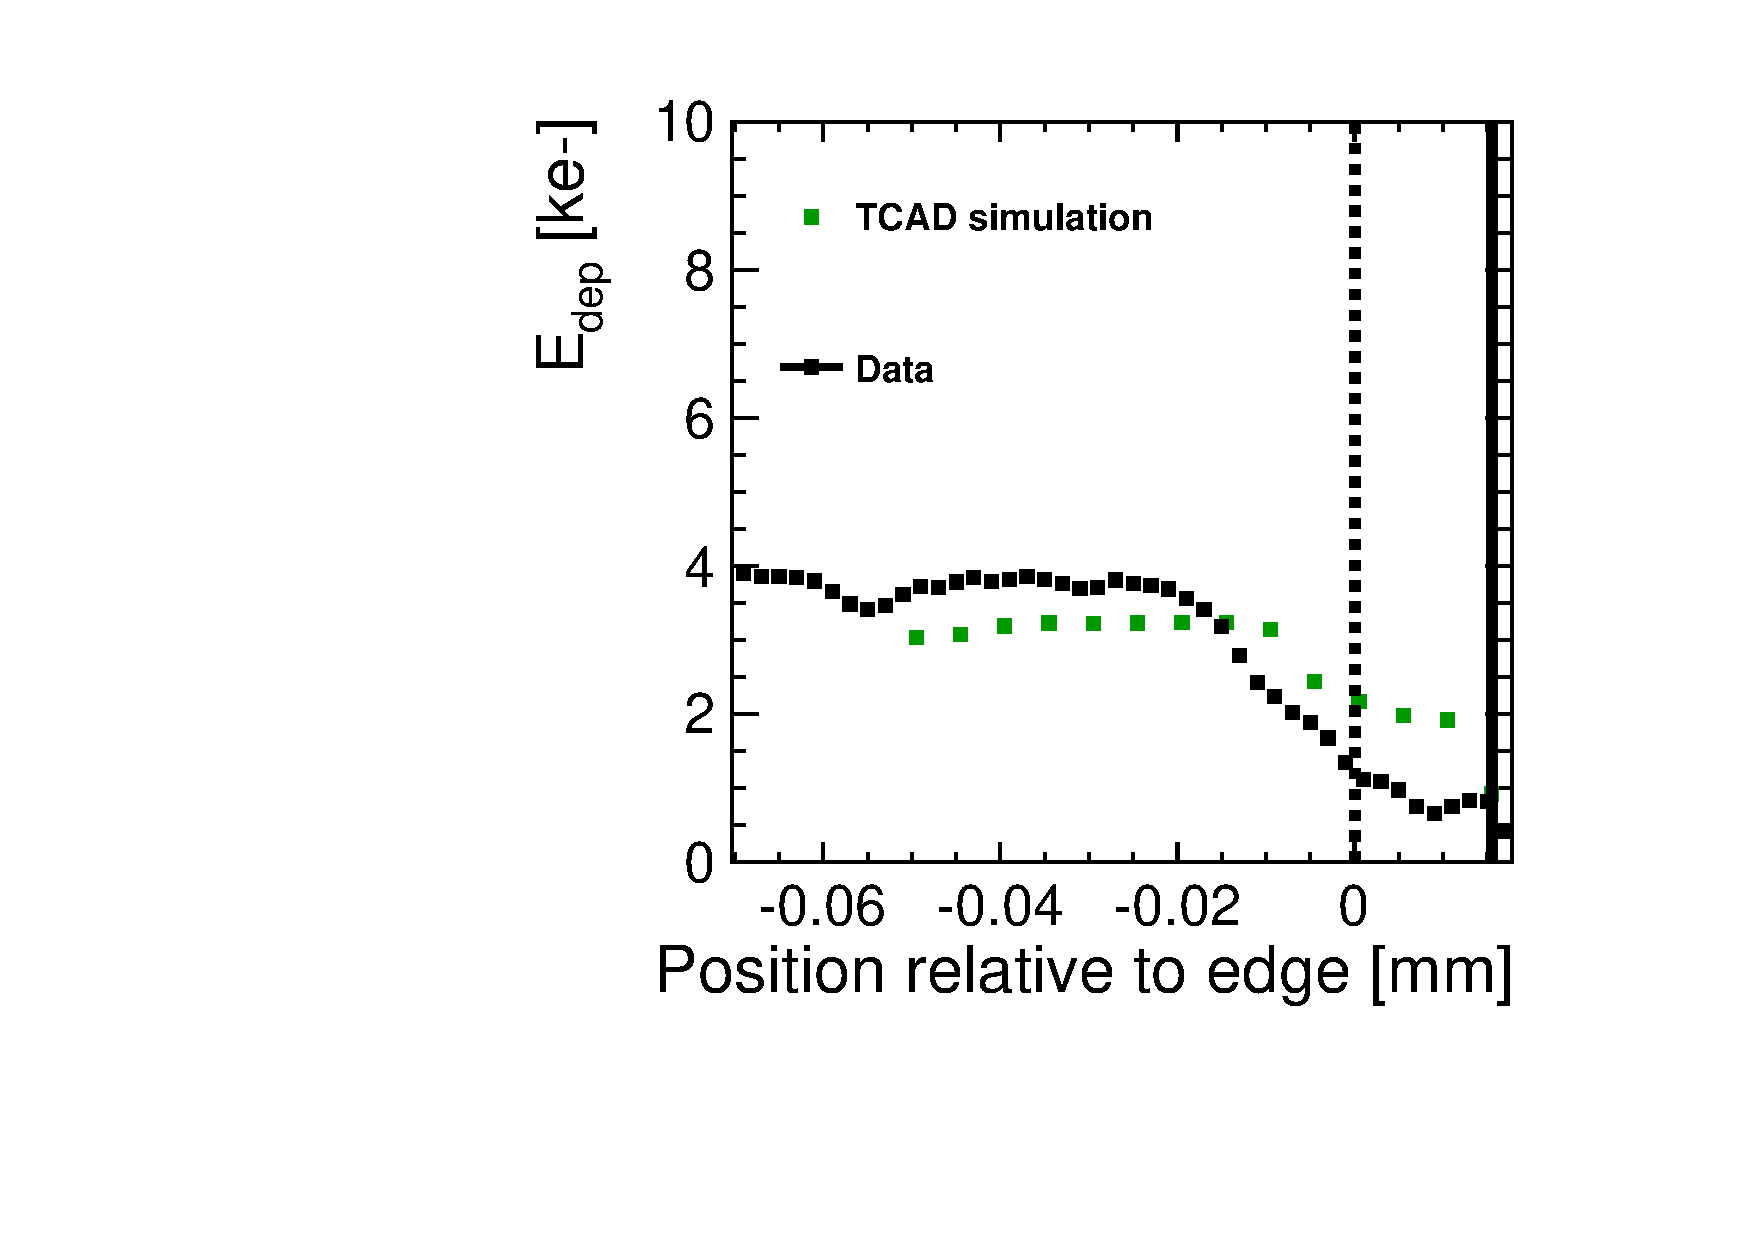
\includegraphics[width=\textwidth]{figures/ActiveEdge/TCAD_data_28_GNDGR.pdf}
    \caption{}
  \end{subfigure}
  \caption{28-GNDGR}
  \label{fig:TCAD_vs_data_28_GNDGR}
\end{figure}


\begin{figure}[htbp]
  \centering
  \begin{subfigure}[b]{0.5\textwidth}
    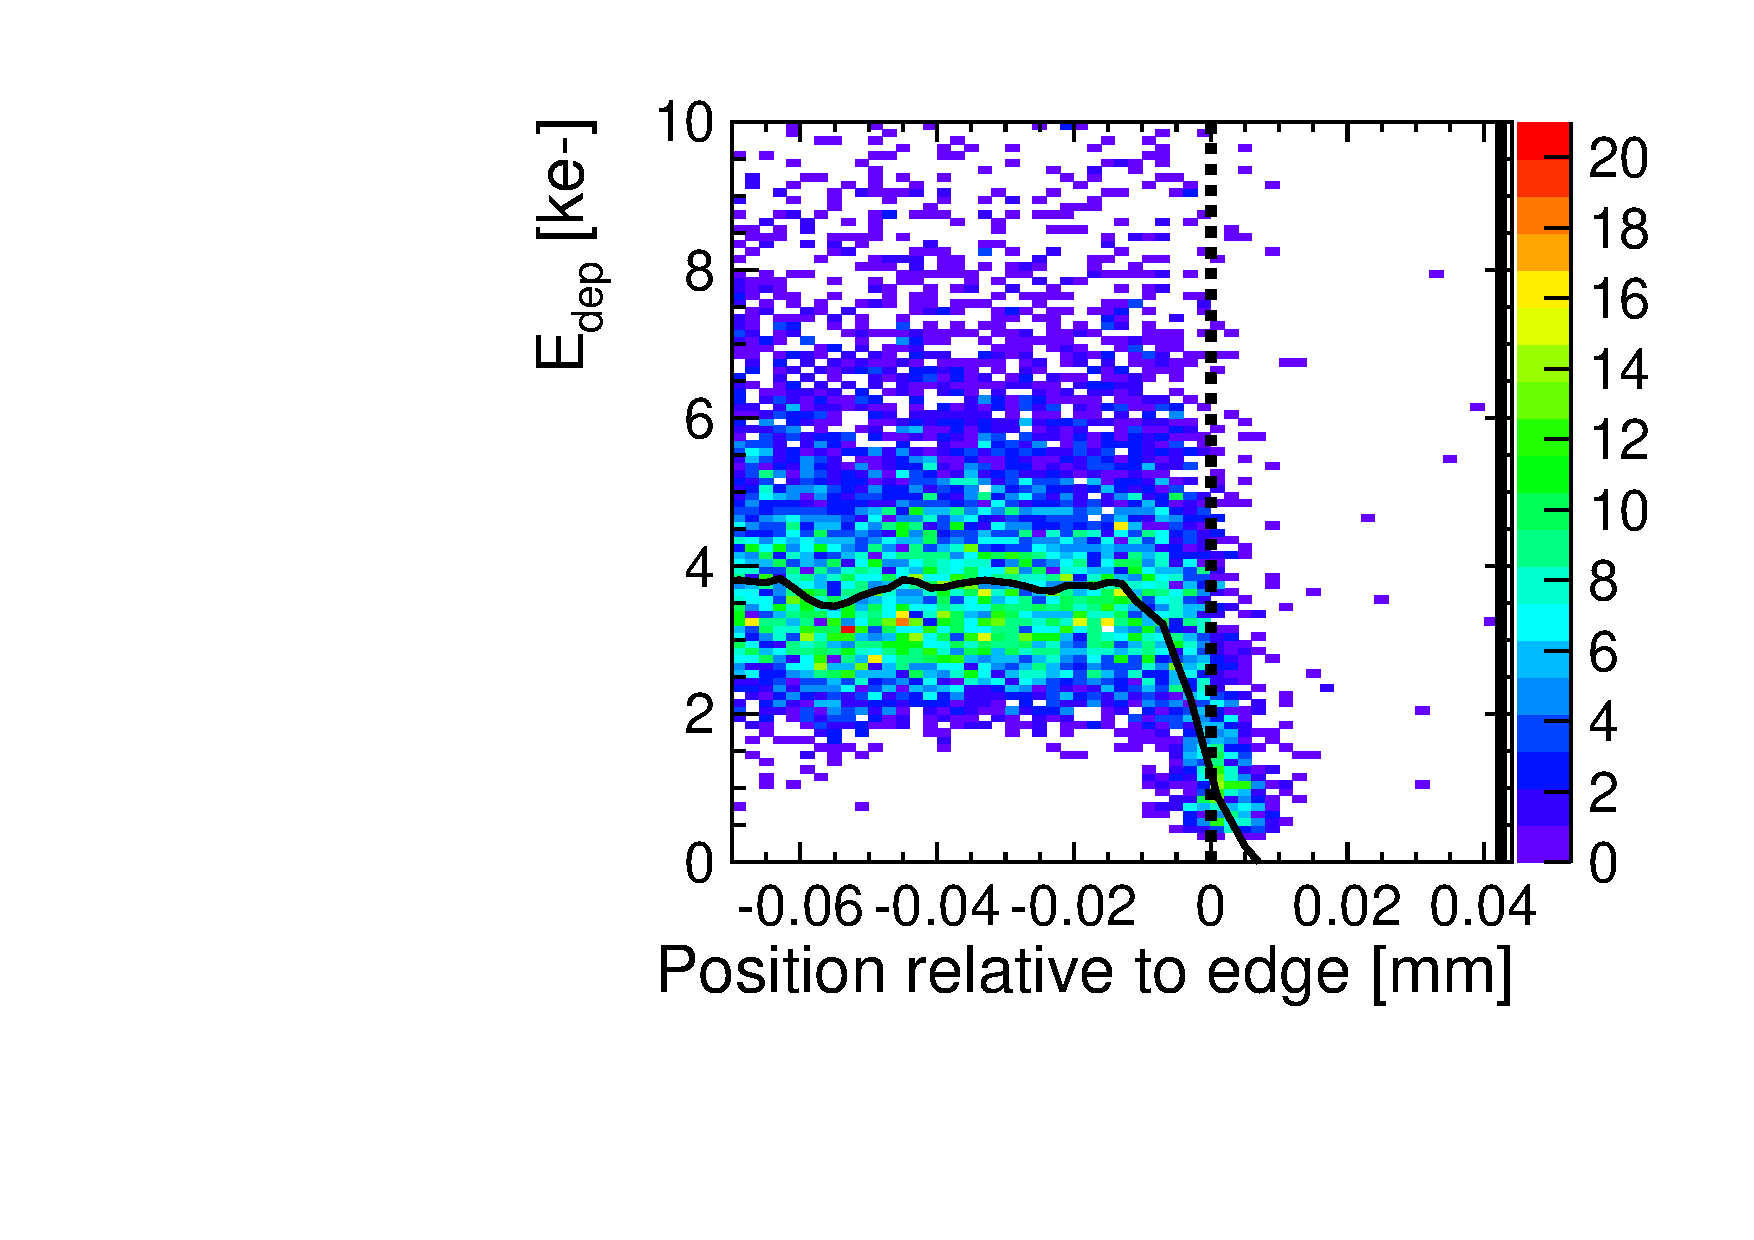
\includegraphics[width=\textwidth]{figures/ActiveEdge/TCAD_data_Edep_55_GNDGR.pdf}
    \caption{}
  \end{subfigure}\hfill
  \begin{subfigure}[b]{0.5\textwidth}
    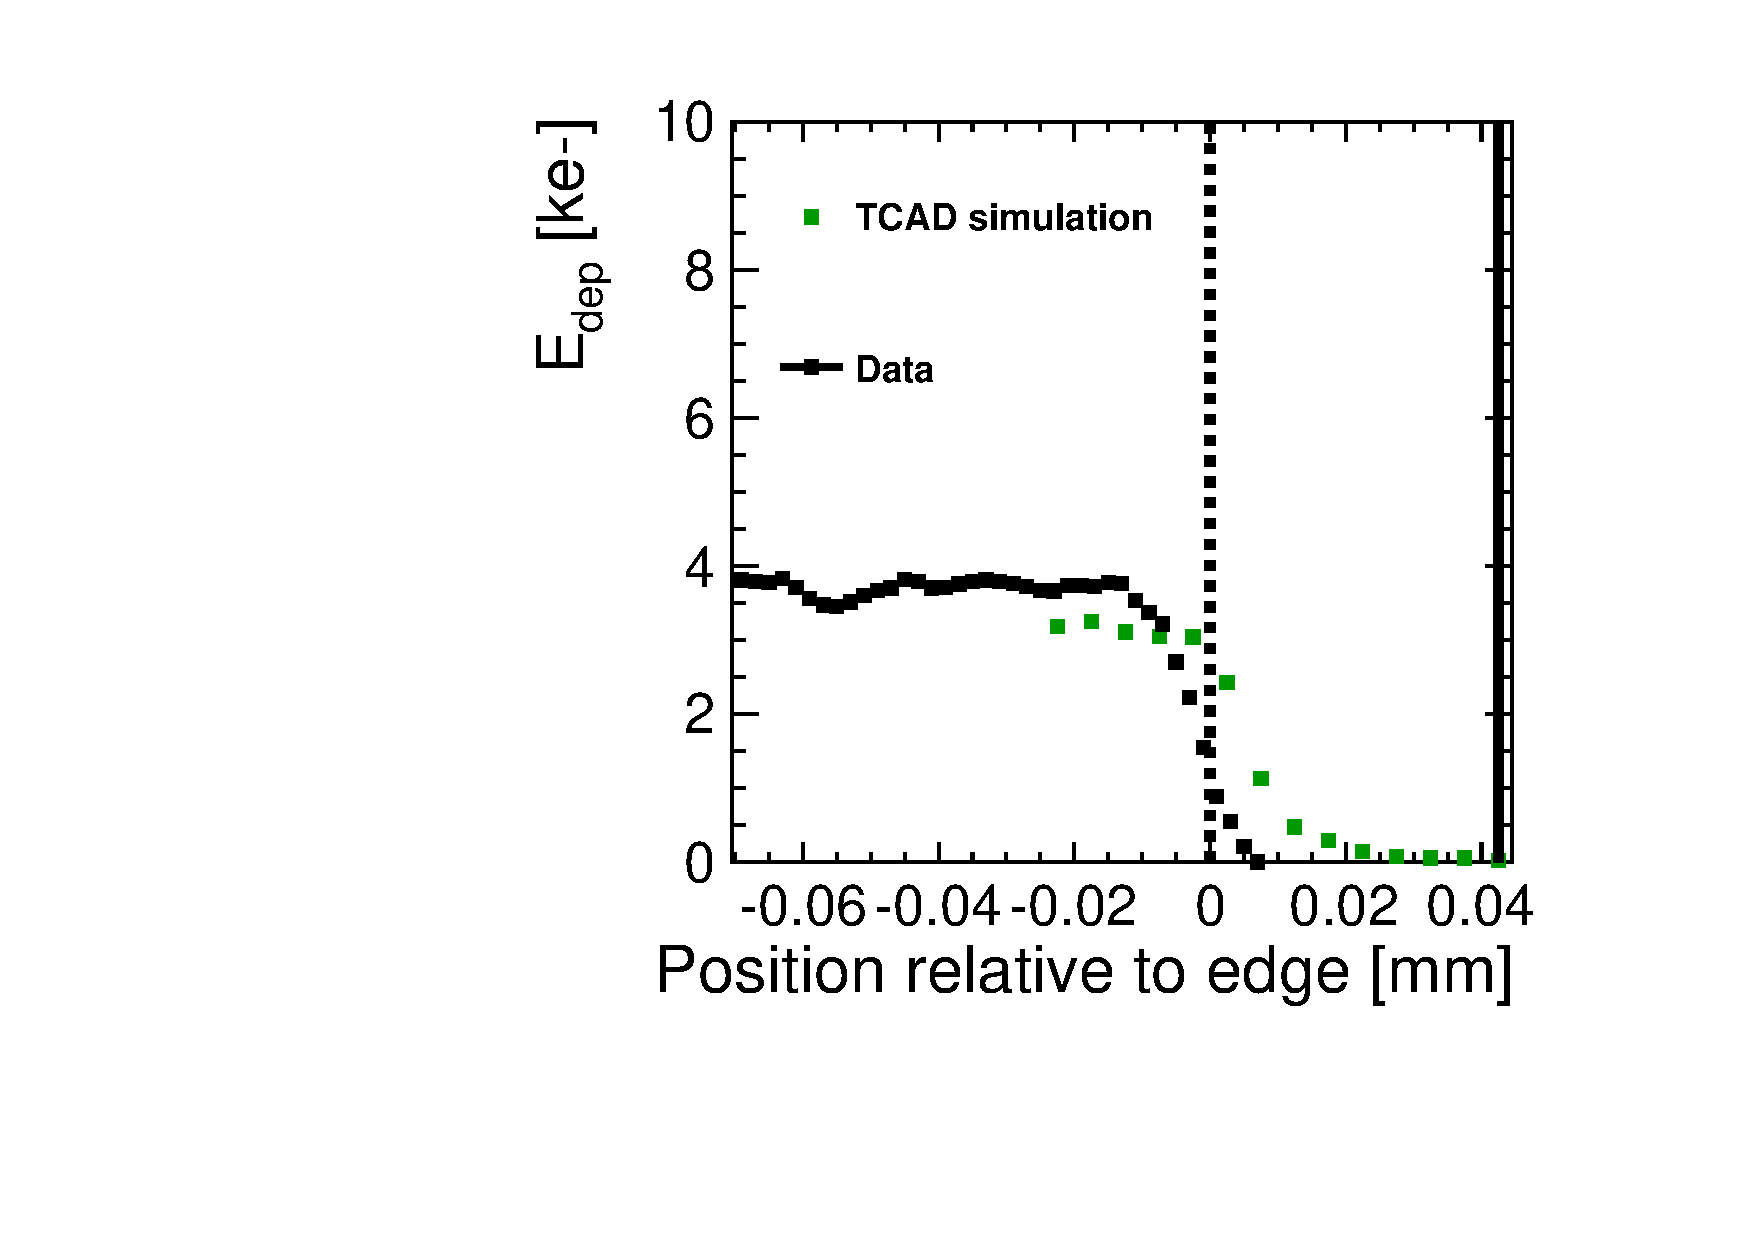
\includegraphics[width=\textwidth]{figures/ActiveEdge/TCAD_data_55_GNDGR.pdf}
    \caption{}
  \end{subfigure}
  \caption{55-GNDGR}
  \label{fig:TCAD_vs_data_55_GNDGR}
\end{figure}

For 55-GNDGR-100 and 55-GNDGR-150 the agreement between data and
simulation is perfect as shown in
\cref{fig:TCAD_vs_data_55_GNDGR_100,fig:TCAD_vs_data_55_GNDGR_150}.

\begin{figure}[htbp]
  \centering
  \begin{subfigure}[b]{0.5\textwidth}
    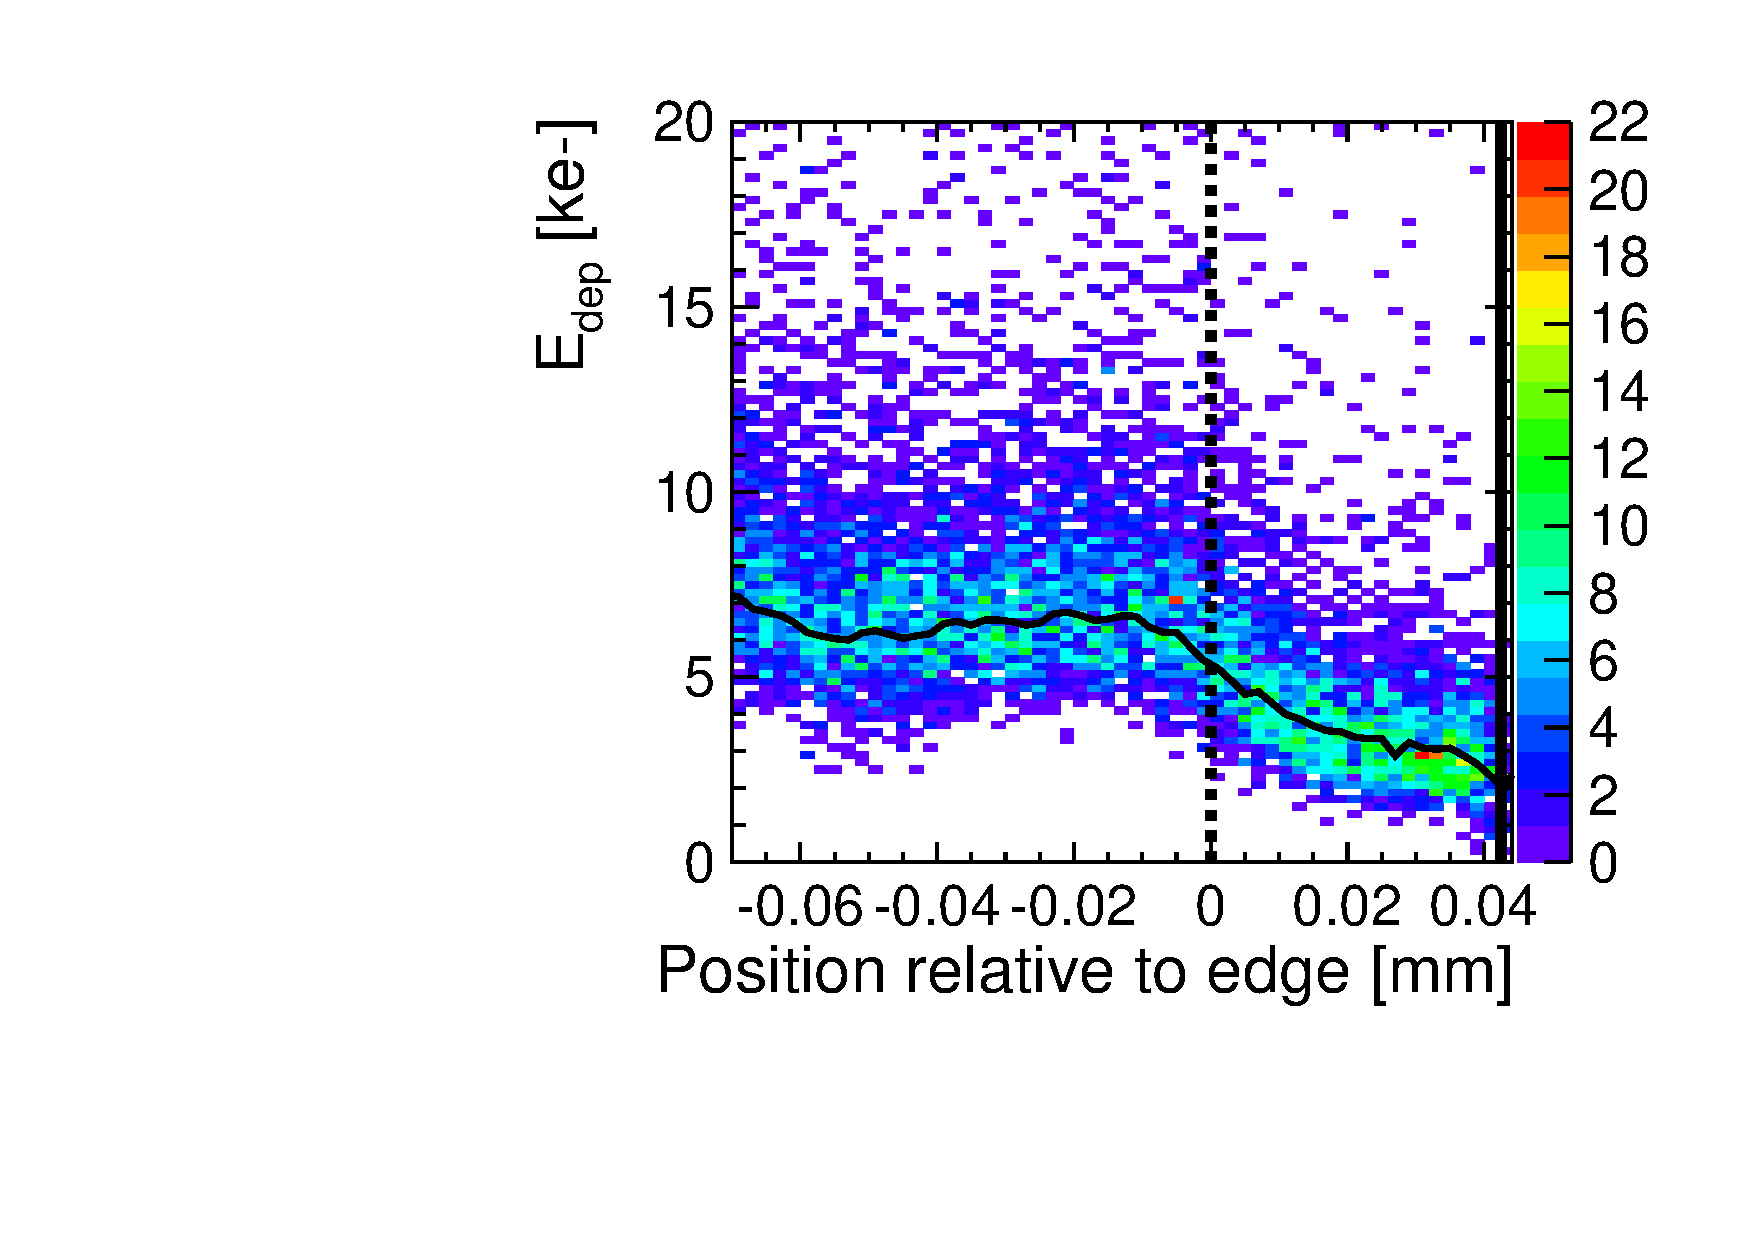
\includegraphics[width=\textwidth]{figures/ActiveEdge/TCAD_data_Edep_55_GNDGR_100.pdf}
    \caption{}
  \end{subfigure}\hfill
  \begin{subfigure}[b]{0.5\textwidth}
    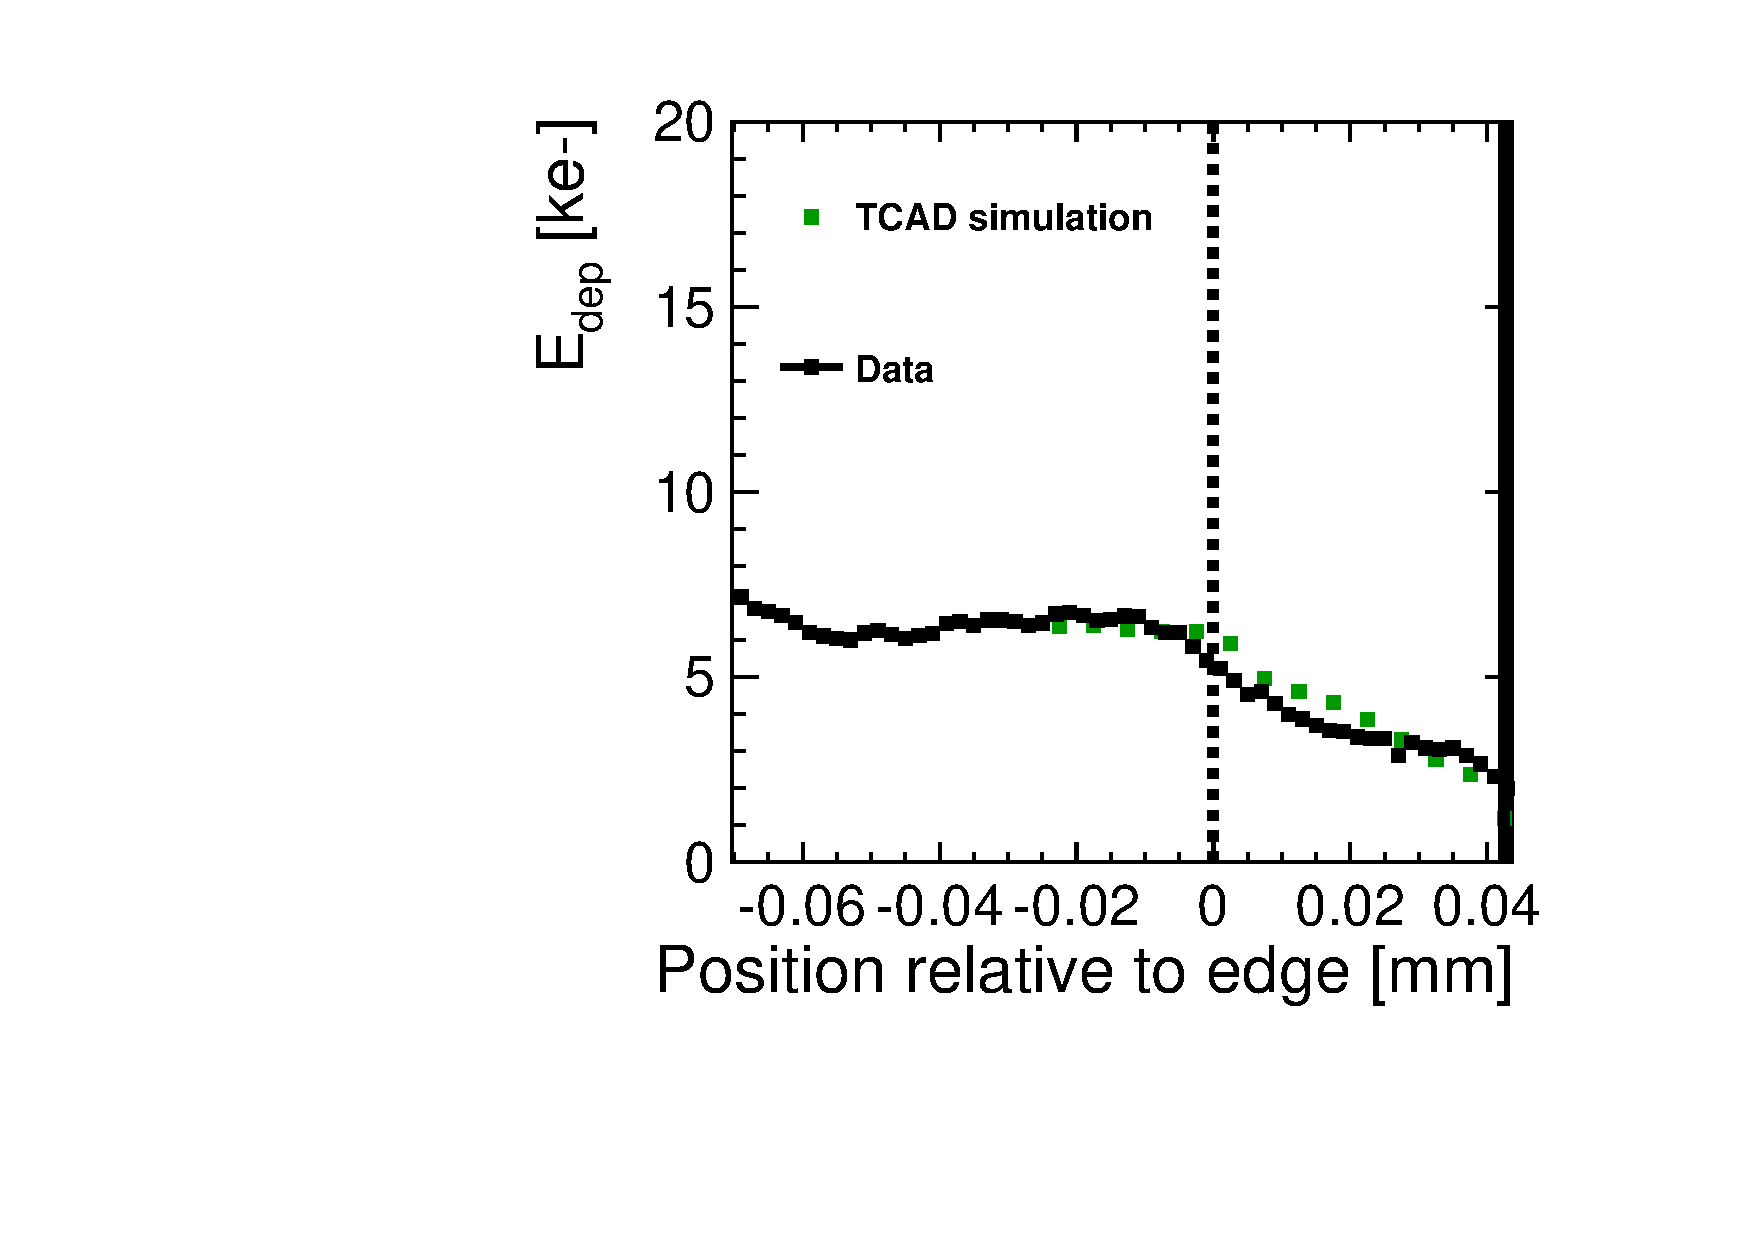
\includegraphics[width=\textwidth]{figures/ActiveEdge/TCAD_data_55_GNDGR_100.pdf}
    \caption{}
  \end{subfigure}
  \caption{55-GNDGR-100}
  \label{fig:TCAD_vs_data_55_GNDGR_100}
\end{figure}



\begin{figure}[htbp]
  \centering
  \begin{subfigure}[b]{0.5\textwidth}
    \includegraphics[width=\textwidth]{figures/ActiveEdge/TCAD_data_Edep_55_GNDGR_150.pdf}
    \caption{}
  \end{subfigure}\hfill
  \begin{subfigure}[b]{0.5\textwidth}
    \includegraphics[width=\textwidth]{figures/ActiveEdge/TCAD_data_55_GNDGR_150.pdf}
    \caption{}
  \end{subfigure}
  \caption{55-GNDGR-150}
  \label{fig:TCAD_vs_data_55_GNDGR_150}
\end{figure}

\cref{fig:TCAD_streamlines} compares the distribution of the
streamlines in the edge for different configurations of guard
rings. The generated charge follows the streamlines and gets collected
by the implants. In the case where there is no guard ring, all the
streamlines reach the first pixel. As confirmed by the data, all the
charge in the edge is collected without any loss. In the case of a
floating guard ring, few streamlines reach the guard ring. This means
some charge is lost in the guard ring instead of being collected by
the first pixel. Finally, in the case of a grounded guard ring more
streamlines end up in the guard ring. This explains also the high drop
in the collected charge in the edge region.

\begin{figure}[htbp]
  \centering
  \begin{subfigure}[b]{\textwidth}
    \includegraphics[width=0.8\textwidth]{figures/ActiveEdge/streamlines_NGR.pdf}
    \caption{No guard ring}
  \end{subfigure}\\
  \begin{subfigure}[b]{\textwidth}
    \includegraphics[width=0.8\textwidth]{figures/ActiveEdge/streamlines_FGR.pdf}
    \caption{Floating guard ring}
  \end{subfigure}\\
  \begin{subfigure}[b]{\textwidth}
    \includegraphics[width=0.8\textwidth]{figures/ActiveEdge/streamlines_GNDGR.pdf}
    \caption{Grounded guard ring}
  \end{subfigure}\\
  \begin{subfigure}[b]{\textwidth}
    \includegraphics[width=0.6\textwidth]{figures/ActiveEdge/streamlines_55-GNDGR-50}
    \caption{55-GNDGR-50}
  \end{subfigure}
  \caption{Streamlines for different configurations of guard ring. The
    generated charges follow the streamlines. The streamlines which
    end up in the guard ring means that those charges are not
    collected by the first pixel and thus lost.}
  \label{fig:TCAD_streamlines}
\end{figure}




%% \newpage
%% \section{Results temp}

%% \begin{figure}[htbp]
%%   \begin{subfigure}[b]{0.24\textwidth}
%%     \centering
%%     \includegraphics[width=\textwidth, page=3]{figures/TestBeam/edge_bcp.pdf}
%%   \caption{}
%%   \end{subfigure}\hfill
%%   \begin{subfigure}[b]{0.24\textwidth}
%%     \centering
%%     \includegraphics[width=\textwidth, page=6]{figures/TestBeam/edge_bcp.pdf}
%%   \caption{}
%%   \end{subfigure}\hfill
%%   \begin{subfigure}[b]{0.24\textwidth}
%%     \centering
%%     \includegraphics[width=\textwidth, page=9]{figures/TestBeam/edge_bcp.pdf}
%%   \caption{}
%%   \end{subfigure}\hfill
%%   \begin{subfigure}[b]{0.24\textwidth}
%%     \centering
%%     \includegraphics[width=\textwidth, page=12]{figures/TestBeam/edge_bcp.pdf}
%%   \caption{}
%%   \end{subfigure}
%%   \caption{}
%%   \label{fig:ResultsTemp}
%% \end{figure}

%% \begin{figure}[htbp]
%%   \begin{subfigure}[b]{0.24\textwidth}
%%     \centering
%%     \includegraphics[width=\textwidth, page=5]{figures/TestBeam/edge_bcp.pdf}
%%   \caption{}
%%   \end{subfigure}\hfill
%%   \begin{subfigure}[b]{0.24\textwidth}
%%     \centering
%%     \includegraphics[width=\textwidth, page=8]{figures/TestBeam/edge_bcp.pdf}
%%   \caption{}
%%   \end{subfigure}\hfill
%%   \begin{subfigure}[b]{0.24\textwidth}
%%     \centering
%%     \includegraphics[width=\textwidth, page=11]{figures/TestBeam/edge_bcp.pdf}
%%   \caption{}
%%   \end{subfigure}\hfill
%%   \begin{subfigure}[b]{0.24\textwidth}
%%     \centering
%%     \includegraphics[width=\textwidth, page=14]{figures/TestBeam/edge_bcp.pdf}
%%   \caption{}
%%   \end{subfigure}
%%   \caption{}
%%   \label{fig:ResultsTemp2}
%% \end{figure}

%% \begin{figure}[htbp]
%%   \begin{subfigure}[b]{0.24\textwidth}
%%     \centering
%%     \includegraphics[width=\textwidth]{figures/ActiveEdge/TCAD_data_Edep_20_NGR.pdf}
%%   \caption{}
%%   \end{subfigure}\hfill
%%   \begin{subfigure}[b]{0.24\textwidth}
%%     \centering

%%   \caption{}
%%   \end{subfigure}\hfill
%%   \begin{subfigure}[b]{0.24\textwidth}
%%     \centering
%%     \includegraphics[width=\textwidth]{figures/ActiveEdge/TCAD_data_Edep_28_GNDGR.pdf}
%%   \caption{}
%%   \end{subfigure}\hfill
%%   \begin{subfigure}[b]{0.24\textwidth}
%%     \centering
%%     \includegraphics[width=\textwidth]{figures/ActiveEdge/TCAD_data_Edep_55_GNDGR.pdf}
%%   \caption{}
%%   \end{subfigure}
%%   \caption{}
%%   \label{fig:ResultsTemp3}
%% \end{figure}


%% %%%%%%%%%%%%%%%%%%%%
%% \begin{figure}[htbp]
%%   \begin{subfigure}[b]{0.45\textwidth}
%%     \centering
%%     \includegraphics[width=\textwidth, page=15]{figures/TestBeam/edge_bcp.pdf}
%%   \caption{}
%%   \end{subfigure}\hfill
%%   \begin{subfigure}[b]{0.45\textwidth}
%%     \centering
%%     \includegraphics[width=\textwidth, page=18]{figures/TestBeam/edge_bcp.pdf}
%%   \caption{}
%%   \end{subfigure}
%%   \caption{}
%%   \label{fig:ResultsTemp4}
%% \end{figure}

%% \begin{figure}[htbp]
%%   \begin{subfigure}[b]{0.45\textwidth}
%%     \centering
%%     \includegraphics[width=\textwidth, page=17]{figures/TestBeam/edge_bcp.pdf}
%%   \caption{}
%%   \end{subfigure}\hfill
%%   \begin{subfigure}[b]{0.45\textwidth}
%%     \centering
%%     \includegraphics[width=\textwidth, page=20]{figures/TestBeam/edge_bcp.pdf}
%%   \caption{}
%%   \end{subfigure}
%%   \caption{}
%%   \label{fig:ResultsTemp5}
%% \end{figure}

%% \begin{figure}[htbp]
%%   \begin{subfigure}[b]{0.45\textwidth}
%%     \centering
%%     \includegraphics[width=\textwidth]{figures/ActiveEdge/TCAD_data_Edep_55_GNDGR_100.pdf}
%%   \caption{}
%%   \end{subfigure}\hfill
%%   \begin{subfigure}[b]{0.45\textwidth}
%%     \centering
%%     \includegraphics[width=\textwidth]{figures/ActiveEdge/TCAD_data_Edep_55_GNDGR_150.pdf}
%%   \caption{}
%%   \end{subfigure}
%%   \caption{}
%%   \label{fig:ResultsTemp6}
%% \end{figure}


%%%%%%%%%%%%%%%%%%%%%%%%%%%%%%%%%%%
% \begin{figure}[htbp]
%   \centering
%   \begin{minipage}[t]{.4\textwidth}
%     \centering
%     \vspace{0pt}
%     \includegraphics[width=0.95\textwidth]{figures/ActiveEdge/pixelLayout_withLayers.png}
%     \caption{}
%     \label{fig:PixelLayout}
%   \end{minipage}
%   \hfill
%   \begin{minipage}[t]{.56\textwidth}
%     \centering
%     \vspace{0pt}
%     \captionof{table}{Layers and dimensions from the gds geometry
%       (taken from Timepix 20um GR FLOAT).}
%     \label{tab:PixelStackDimensions}
%     \begin{tabular}{l c c}
%       \toprule
%       Layer number & Layer & Diameter [\micron]\\
%       \midrule
%       6 & metal & 36 \\
%       3 & - & 34.62 \\
%       8 & implant & 30 \\
%       9 & UBM (for thin film lift off metal) (??) & 25.6 \\
%       15 & passivation & 19.5 \\
%       5 & contact to connect Al to Si & 15 \\
%       \bottomrule
%     \end{tabular}
%   \end{minipage}
% \end{figure}




% \begin{figure}[htbp]
%   \centering
%   \begin{subfigure}[b]{0.33\textwidth}
%     \centering
%     \fbox{\includegraphics[width=0.95\textwidth]{figures/ActiveEdge/20umEdge_float_GR_withText.png}}
%     \caption{20~\micron edge: Floating guard ring}
%     \label{fig:GuardRingLayout_20_float_GR}
%   \end{subfigure}\hfill
%   \centering
%   \begin{subfigure}[b]{0.33\textwidth}
%     \centering
%     \fbox{\includegraphics[width=0.95\textwidth]{figures/ActiveEdge/20umEdge_GND_GR_withText.png}}
%     \caption{20~\micron edge: GND guard ring}
%     \label{fig:GuardRingLayout_20_GND_GR}
%   \end{subfigure}\hfill
%   \centering
%   \begin{subfigure}[b]{0.33\textwidth}
%     \centering
%     \fbox{\includegraphics[width=0.95\textwidth]{figures/ActiveEdge/50umEdge_GND_GR_withText.png}}
%     \caption{50~\micron edge: GND guard ring}
%     \label{fig:GuardRingLayout_50_GND_GR}
%   \end{subfigure}
%   \label{fig:GuardRingLayout}
% \end{figure}


% For the 50~\micron grounded GR, the dimensions of the pixels are
% differente from above.
% \captionof{table}{Layers and dimensions from the gds geometry
%   (taken from Timepix 20um GR FLOAt and from Timepix 50~\micron grounded GR).}
% \label{tab:PixelStackDimensions}
% \begin{tabular}{l c c c}
%   \toprule
%   Layer number & Layer & Diameter (20 float) [\micron] & Diameter (50 GND) [\micron]\\
%   \midrule
%   6 & metal & 36 & 40 \\
%   3 & - & 34.62 & 36 \\
%   8 & implant & 30 & 30 \\
%   9 & UBM & 25.6 & 25.6 \\
%   15 & passivation & 19.5 & 19.5 \\
%   5 & contact to connect Al to Si & 15 & 15 \\
%   \bottomrule
% \end{tabular}






% For the $50\,\micron$ thick sensors, 4 edge configurations are
% studied: 
% \begin{itemize}
% \item 20-NGR does not contain any guard-ring in the edge with an edge
%   distance of $20\,\micron$.
% \item 23-FGR contains a guard ring with a floating potential. The
%   edge distance is $23\,\micron$.
% \item 28-GNDGR contains a guard ring connected to the ground potential
%   with an edge distance of $28\,\micron$.
% \item 55-GNDGR contains a guard ring connected to the ground potential
%   with an edge distance of $55\,\micron$.
% \end{itemize}

% For 55-GNDGR-100 ($100\,\micron$ thick sensor) and 55-GNDGR-150
% ($150\,\micron$ thick sensor), the edge contains a guard ring
% connected to the ground potential with an edge distance of
% $55\,\micron$.

% \begin{table}[htbp]
%   \centering
%   \caption{Advacam active-edge n-in-p planar pixel sensor assemblies. The edge distance is defined by the distance between the last pixel implant and the physical sensor edge.}
%   \label{tab:activeEdgeAssembliesList}
%   \begin{tabular}{lccc}
%     \toprule
%     Assembly & Thickness [\micron] & Edge distance [\micron] & ID \\
%     \midrule
%     20-NGR  & 50 & 20 & W19\_G7 \\
%     23-FGR & 50 & 23 & W19\_F7 \\
%     28-GNDGR & 50 & 28 & W19\_L8 \\
%     55-GNDGR & 50 & 55 &W19\_C7 \\ \hline
%     55-GNDGR-100 & 100 & 55 & W5\_E2  \\ \hline
%     55-GNDGR-150 & 150 & 55 & W5\_F1 \\
%     \bottomrule
%   \end{tabular}
% \end{table}
